\documentclass[12pt, a4paper]{book}
\begin{document}\label{chap:Best_ML}
Something something Time to prepare our ML algorithms, statistics etc..

\section{Neural Network Training}
For most of the NN optimization methods we trained a NN with the following hyperparameters:
\begin{itemize}
   \item One hidden layer
   \item 100 neurons in the hidden layer
   \item 0.1 learning rate $\eta$
   \item $10^{-5}$ L2-regularization parameter $\lambda$
   \item The ADAM optimizer
\end{itemize}
We will mention whenever these parameters were not used. The results for the different network optimization methods explained in Chapter \ref{chap:NN_train} follow from here. Startngg with the normalization of data.\\

\clearpage

\subsection{Normalization of data}\label{sec:normie_NN_res}
We trained a network using 80\% of the whole SM background events as well as 80\% of all the Z' DH HDS samples. As sample weights we only balanced the signal and background using MC events. We did this by using method 3. on Chapter \ref{sec:balance_NN}. 
We tested on the remaining 20\% of the SM background events, as well as 20\% of Z' DH HDS events where $m_{Z'} =130$ GeV. The different normalization methods explained in Chapter \ref{sec:normie_NN} have been tested and can be seen in the Figure \ref{fig:DifferentNormalizations}. \\
\graphicspath{{../../../Plots/NeuralNetwork/Normalization_method/}}
\begin{figure}[!ht]
	\centering
	\begin{subfigure}[b]{0.49\textwidth}
      \centering
      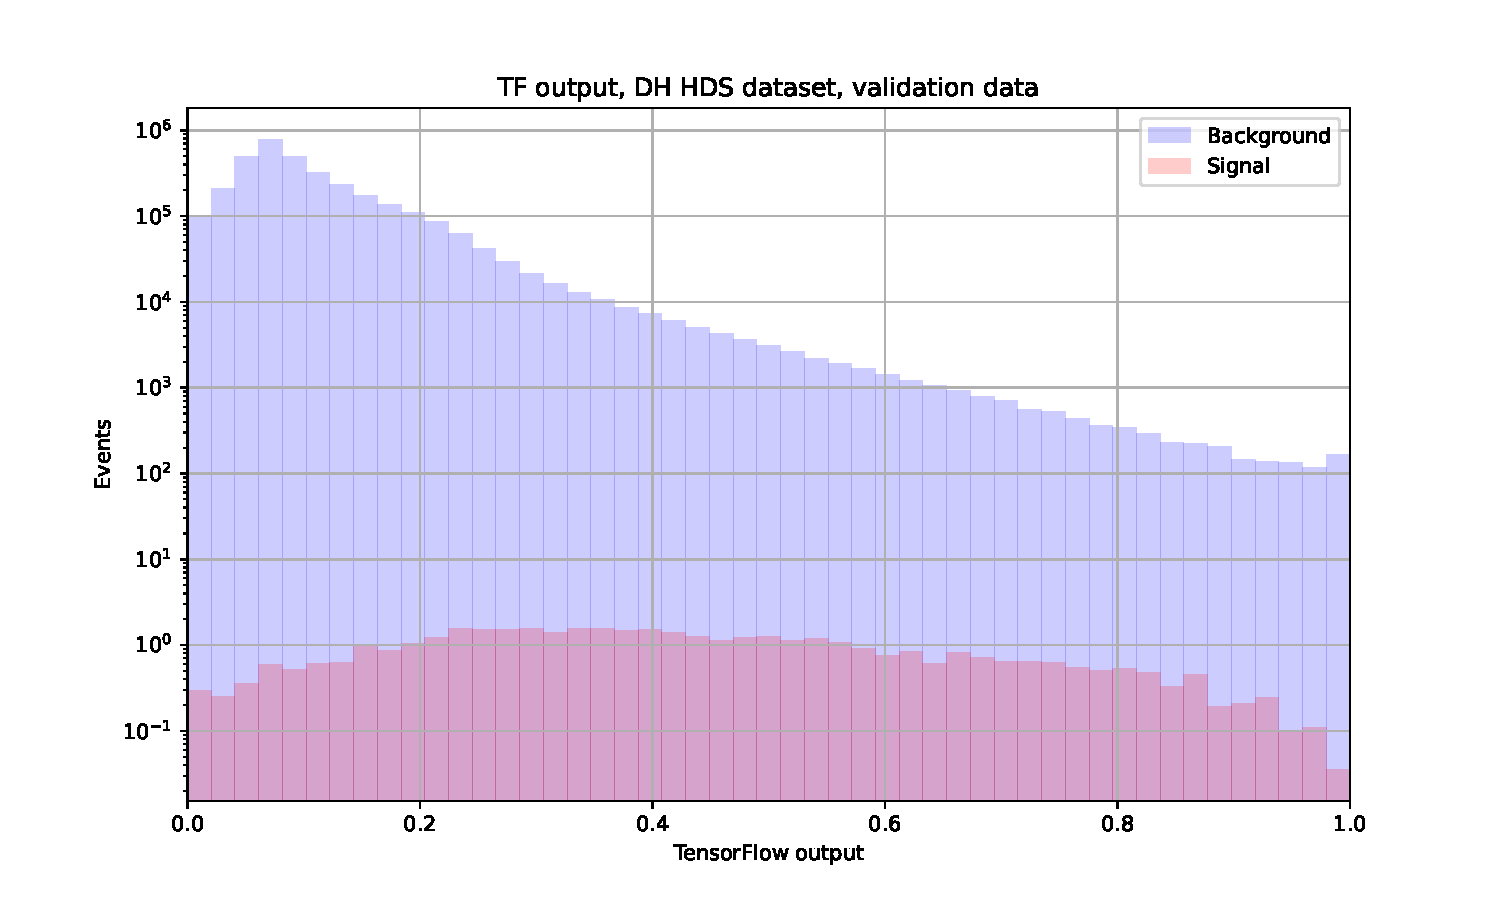
\includegraphics[width=1\textwidth]{NoNorm/VAL_pre.pdf}
      \caption{No normalization}
   \end{subfigure}
   \hfill
   \begin{subfigure}[b]{0.49\textwidth}
      \centering
      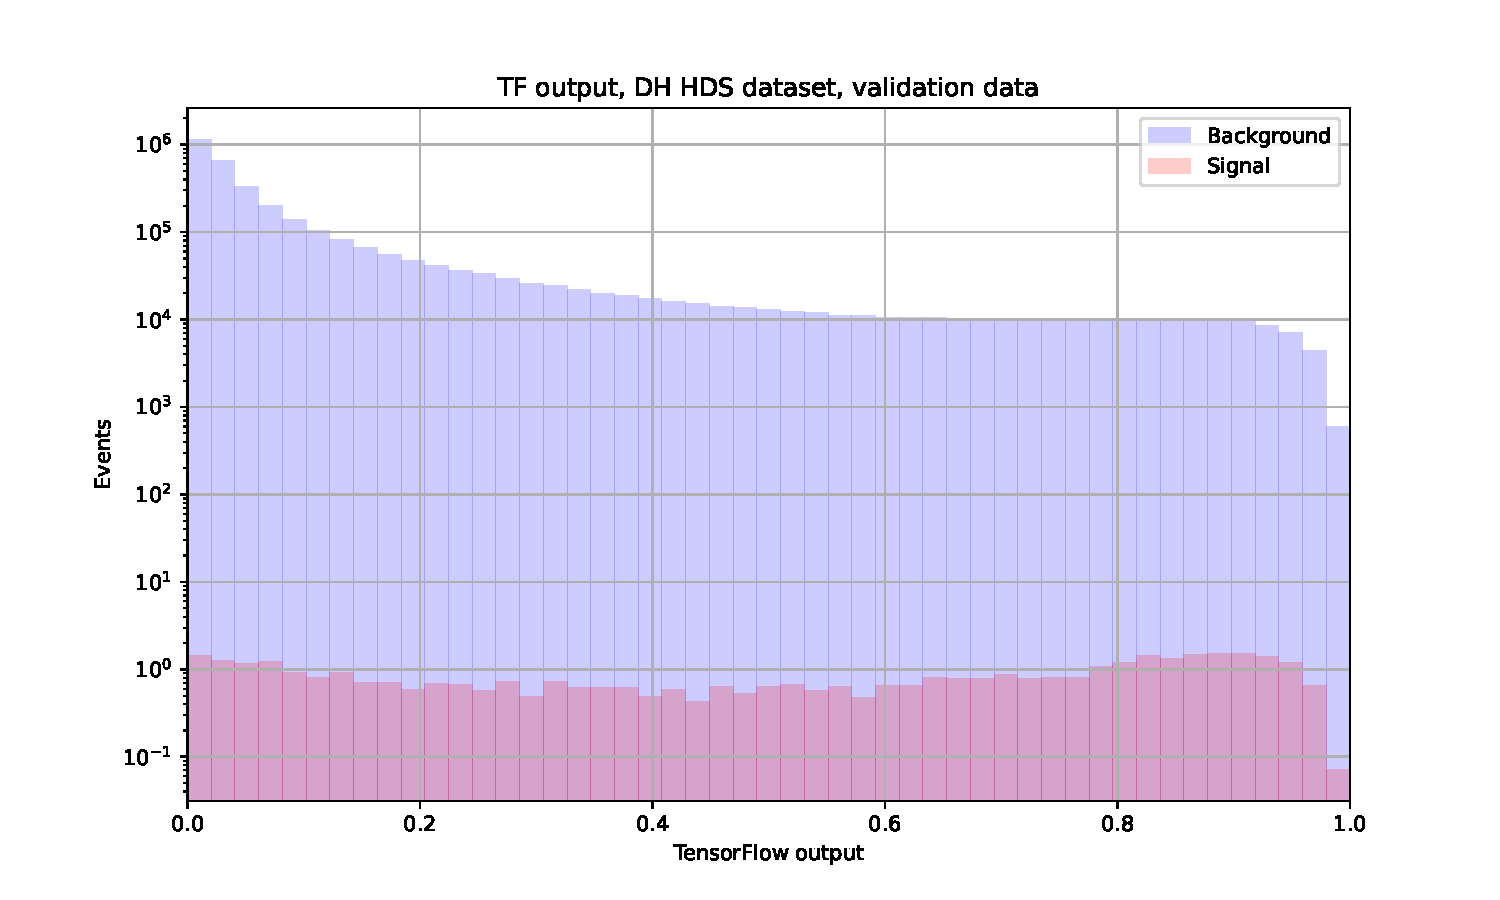
\includegraphics[width=1\textwidth]{LayerNorm/VAL_pre.pdf}
      \caption{Layer normalization}
   \end{subfigure}
   \hfill
	\begin{subfigure}[b]{0.49\textwidth}
      \centering
      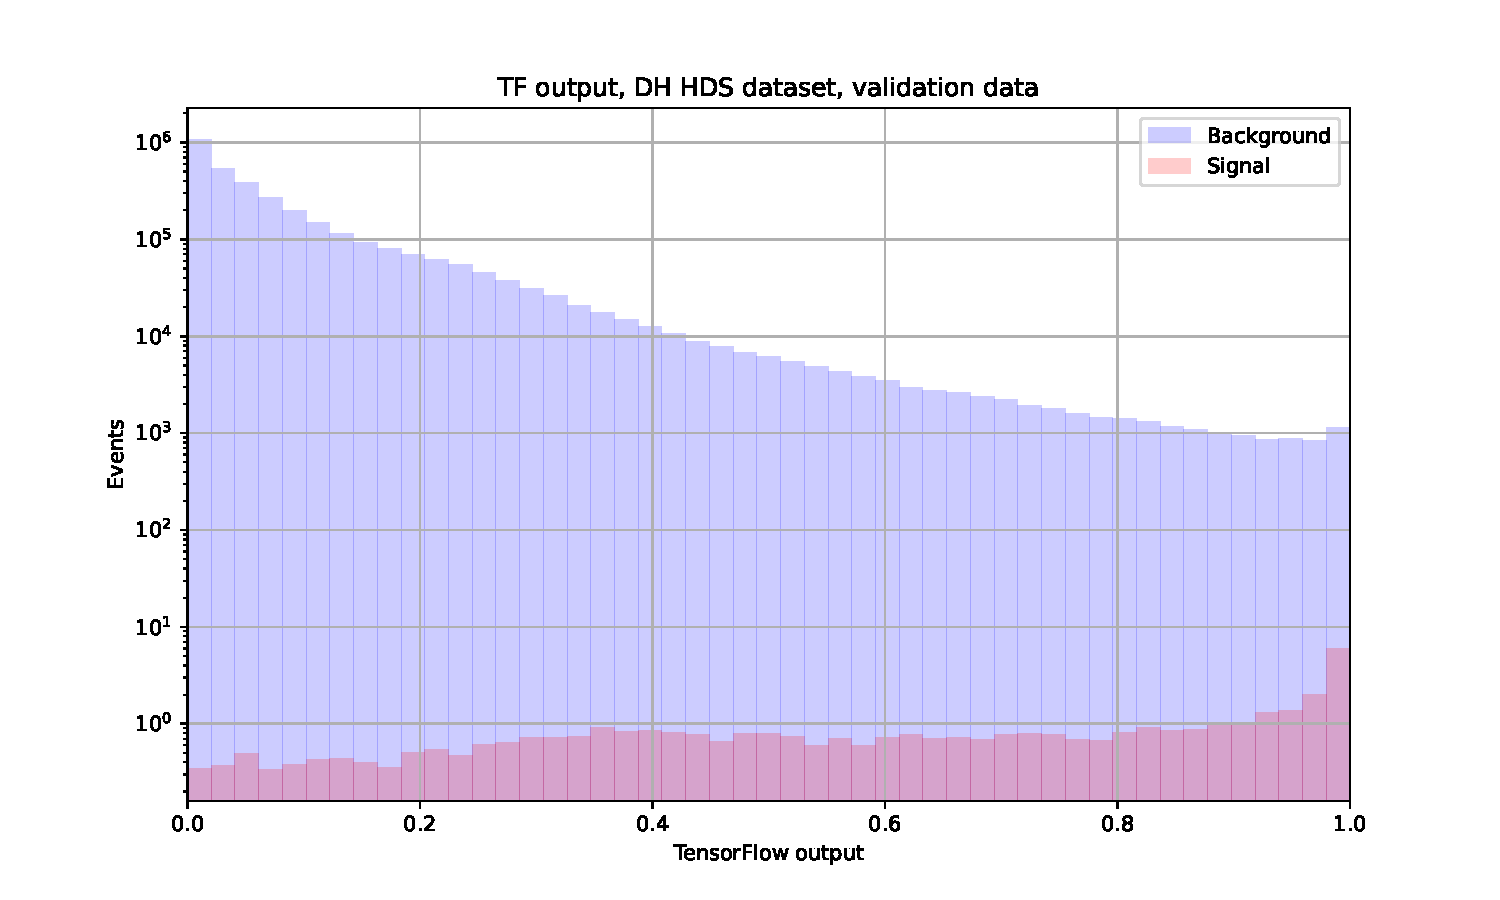
\includegraphics[width=1\textwidth]{minmax/VAL_pre.pdf}
      \caption{Min max scaling}
   \end{subfigure}
   \hfill
   \begin{subfigure}[b]{0.49\textwidth}
      \centering
      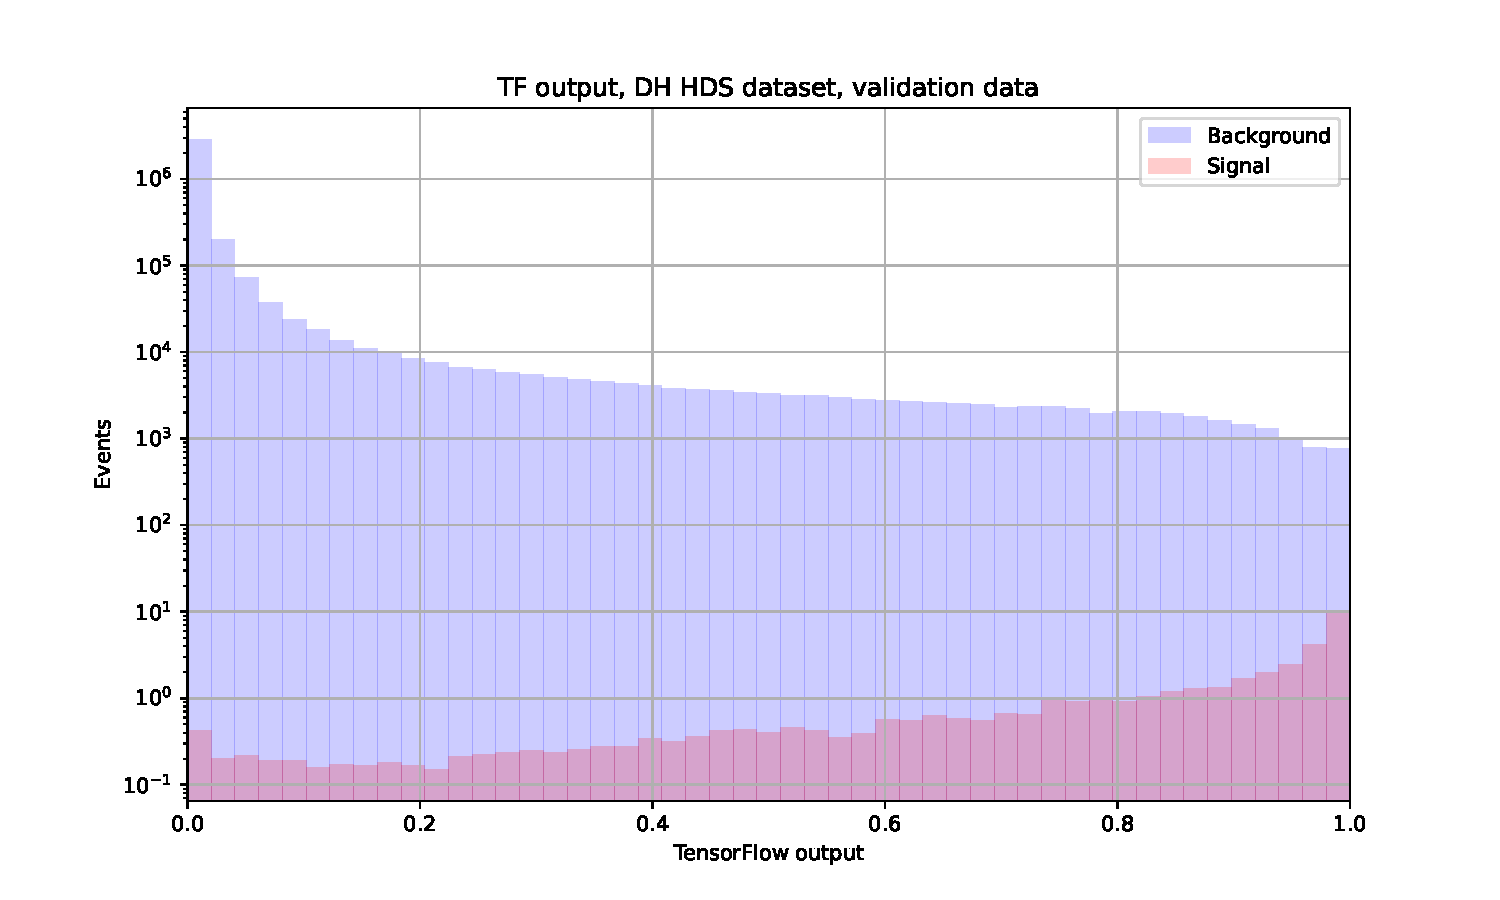
\includegraphics[width=1\textwidth]{Z_score/VAL_pre.pdf}
      \caption{Z-score}
   \end{subfigure}
   \hfill
   \begin{subfigure}[b]{0.49\textwidth}
      \centering
      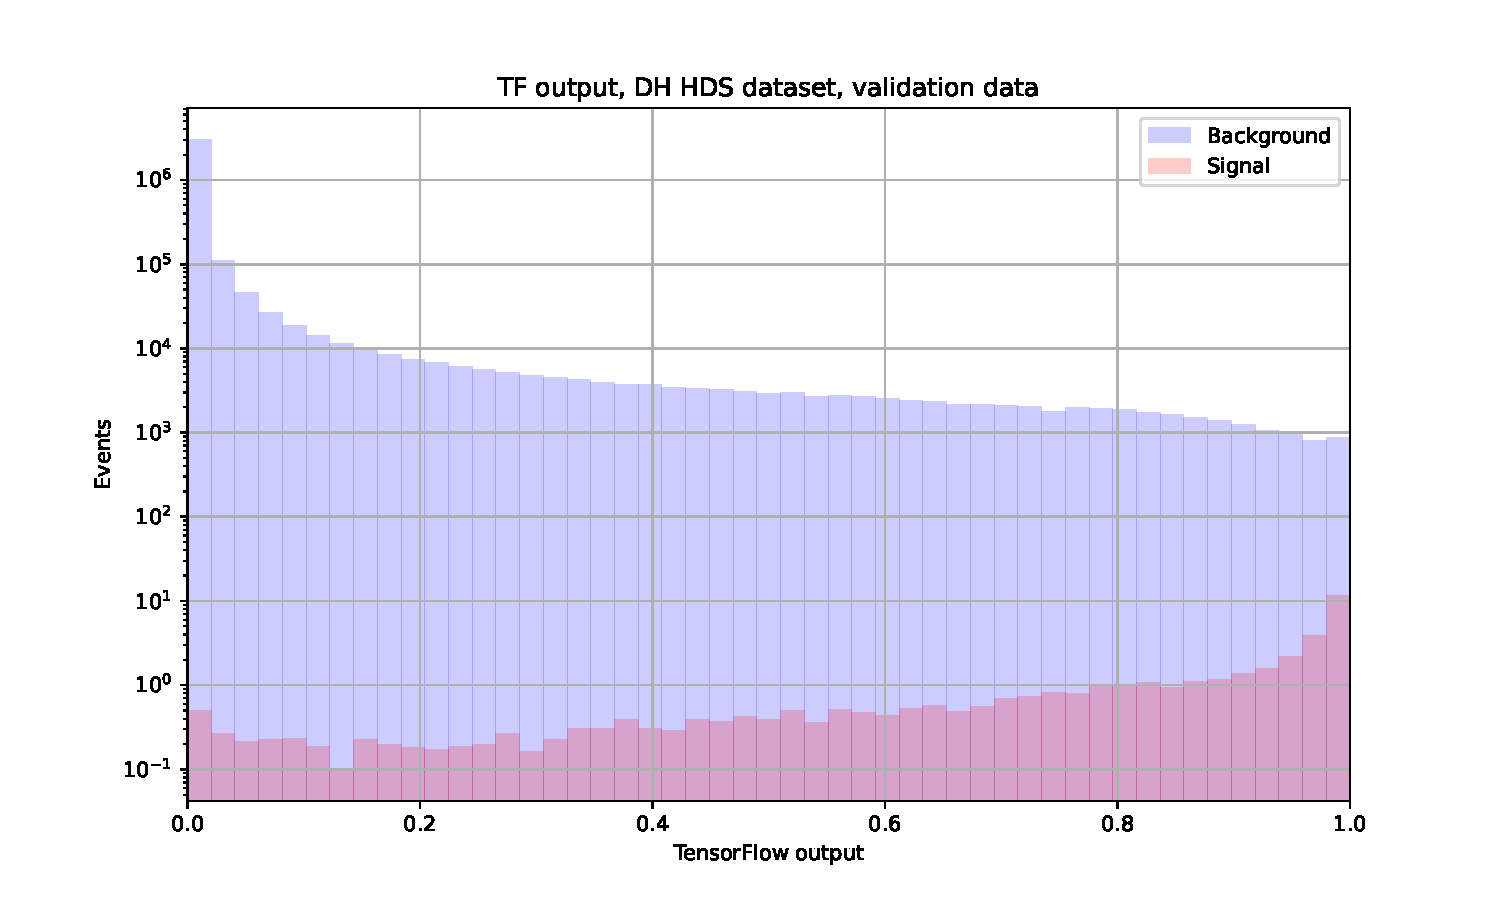
\includegraphics[width=1\textwidth]{BatchNorm/VAL_pre.pdf}
      \caption{Batch normalization}
   \end{subfigure}
   \caption[Different normaliazation methods for NNs]{NN prediction when using different normalization methods. This is testing a dataset with 20\% of the Z' DH HDS $m_{Z'}=130$ GeV events.}\label{fig:DifferentNormalizations}
\end{figure}
\\Inclduing datapoints as well as uncertainties on the best performing normalizatin methods, as well as their calculate expected significance as explained in Chapter \ref{sec:siggy}, yields the plots
shown in Figure \ref{fig:BestNormie}. For more Figures showing NN training results see the GitHub repo\footnote{Available here: \href{https://github.com/rubenguevara/Master-Thesis/tree/master/Plots/NeuralNetwork/Normalization_method}{https://github.com/rubenguevara/Master-Thesis/tree/master/\\Plots/NeuralNetwork/Normalization\_method}}. 
\begin{figure}[!ht]
	\centering
	\begin{subfigure}[b]{0.49\textwidth}
      \centering
      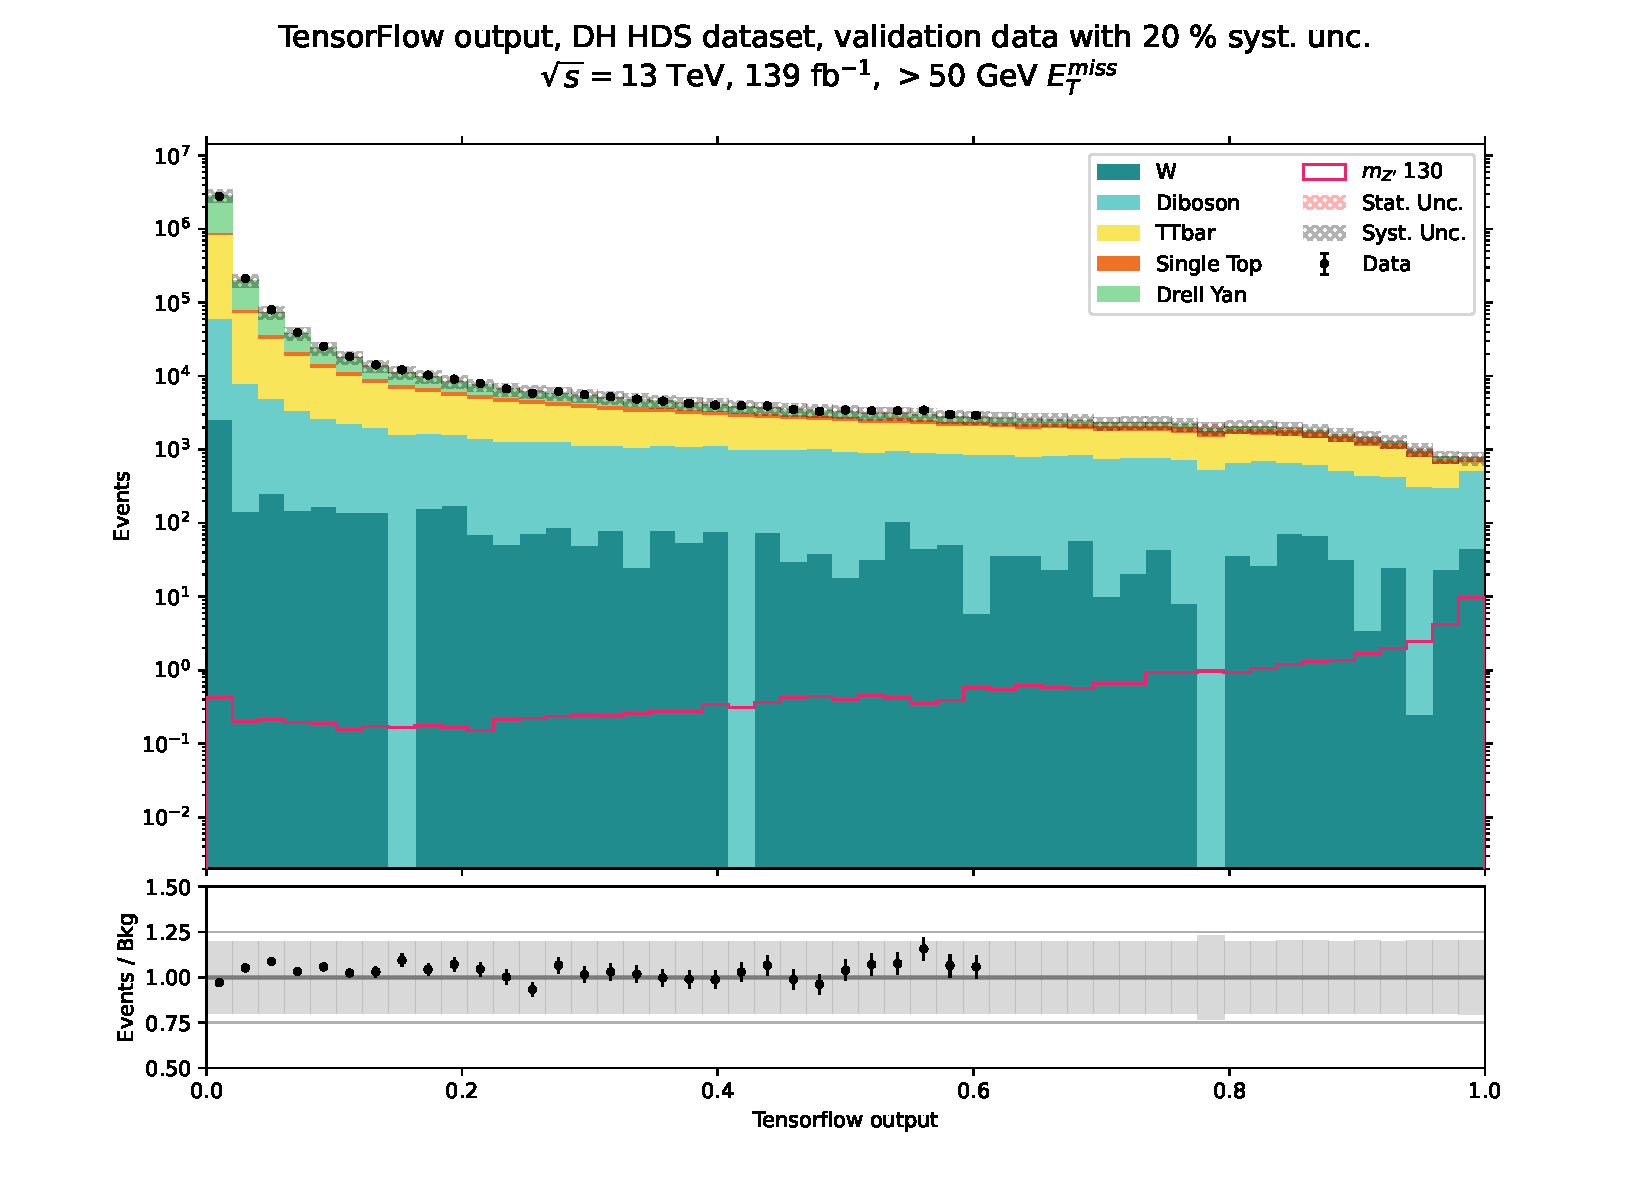
\includegraphics[width=1\textwidth]{Z_score/VAL.pdf}
      \caption{Z-score}
   \end{subfigure}
   \hfill
   \begin{subfigure}[b]{0.49\textwidth}
      \centering
      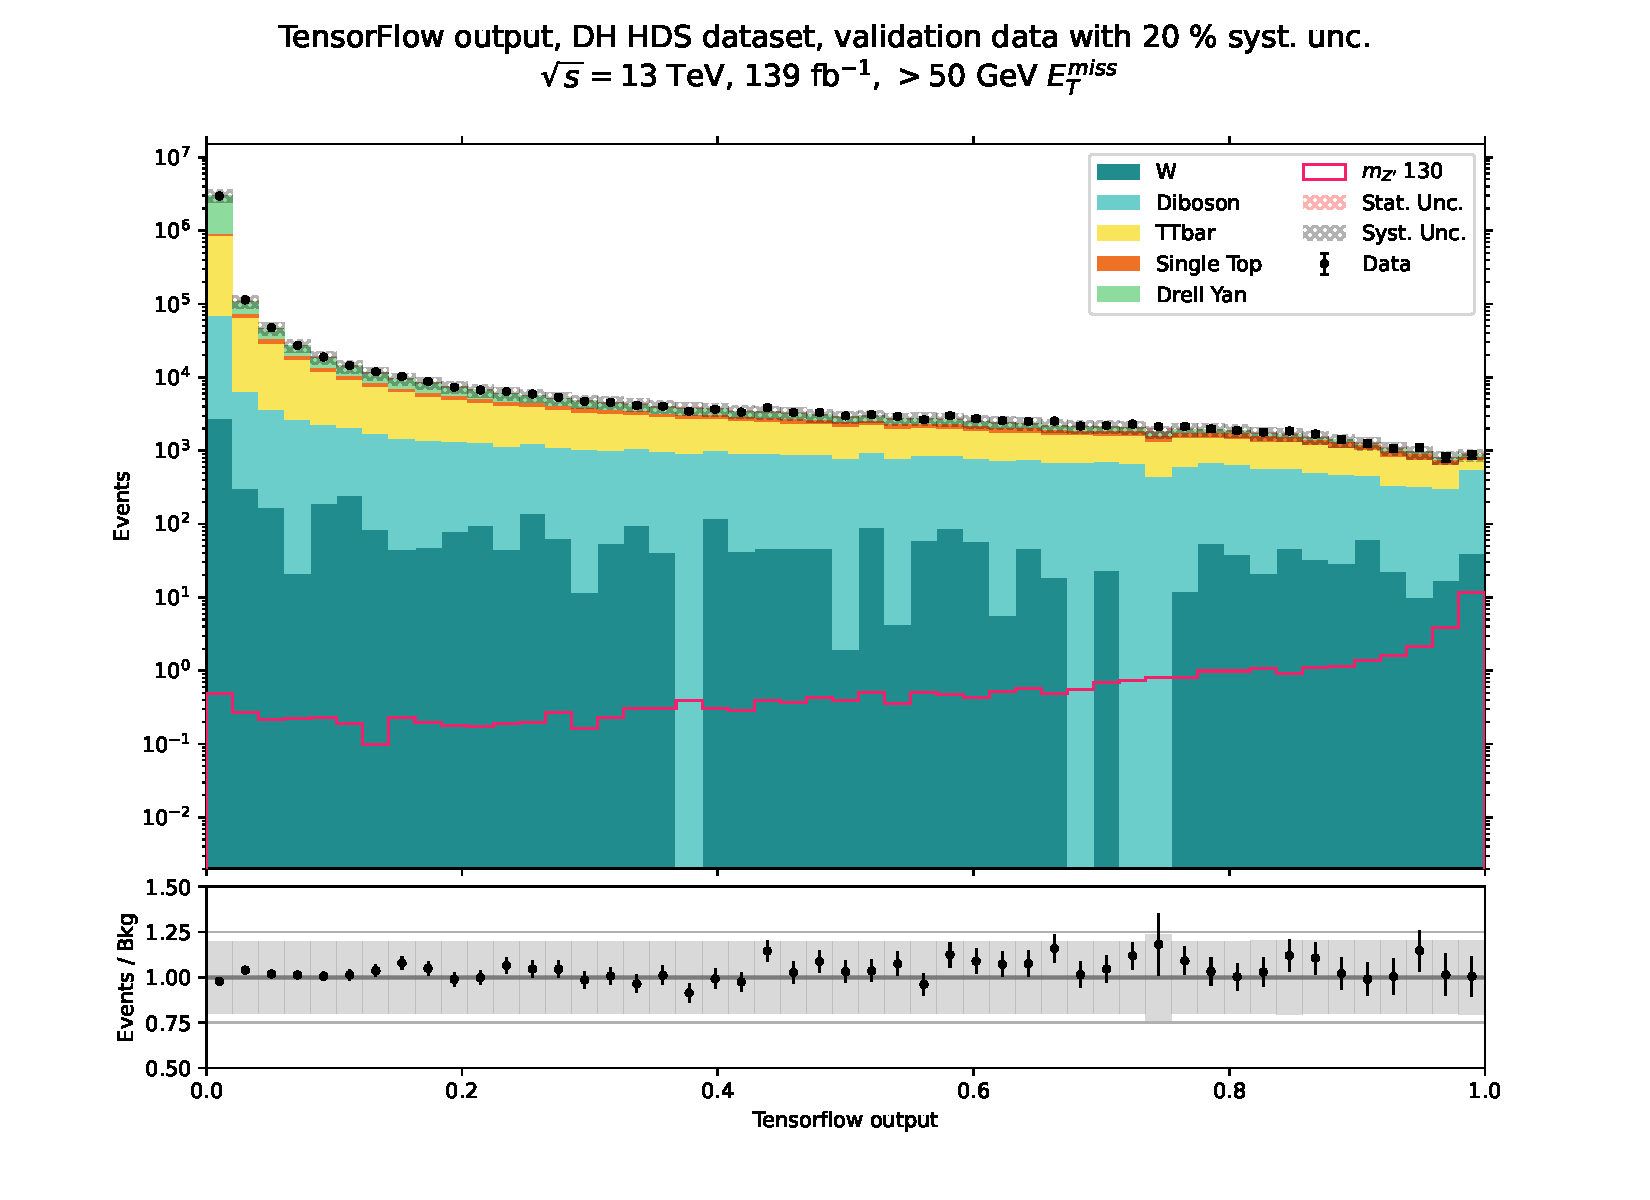
\includegraphics[width=1\textwidth]{BatchNorm/VAL.pdf}
      \caption{Batch normalization}
   \end{subfigure}
   \hfill
   \begin{subfigure}[b]{0.49\textwidth}
      \centering
      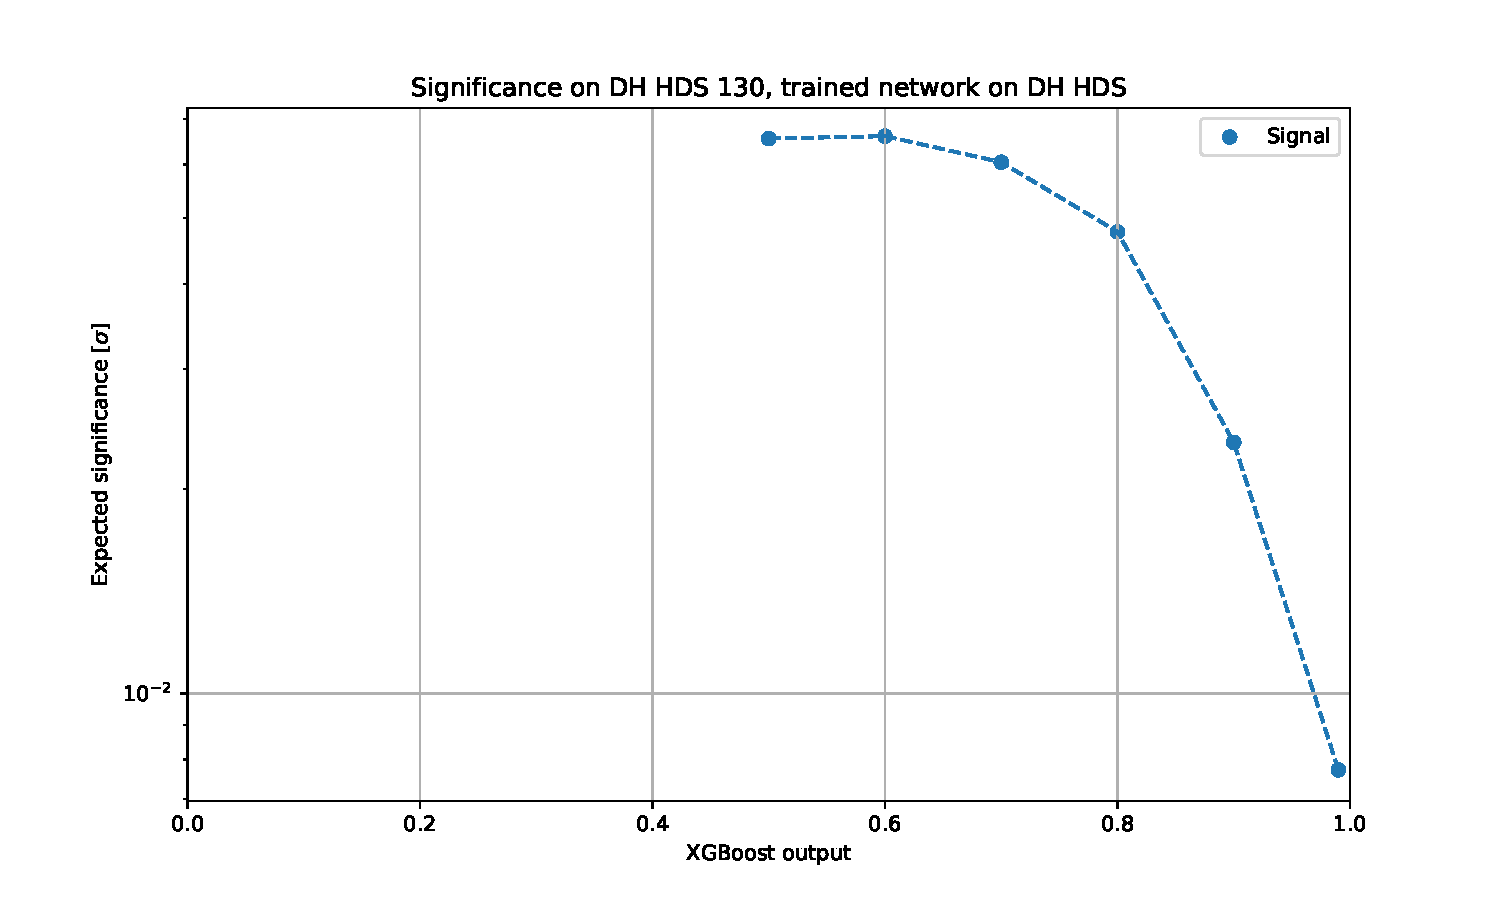
\includegraphics[width=1\textwidth]{Z_score/EXP_SIG.pdf}
      \caption{The expected significance of a)}
   \end{subfigure}
   \hfill
   \begin{subfigure}[b]{0.49\textwidth}
      \centering
      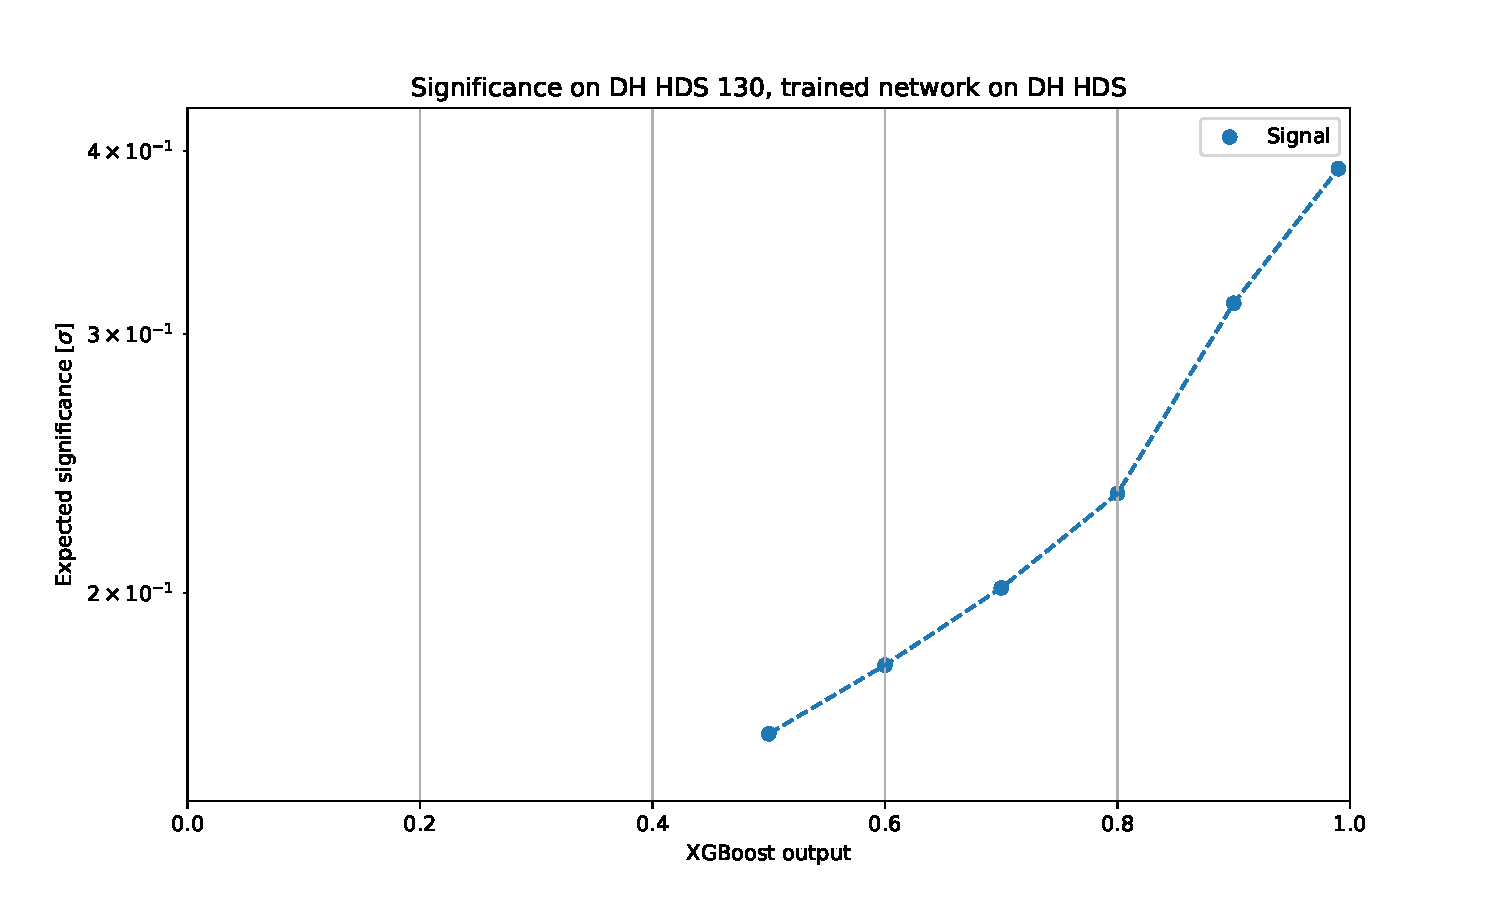
\includegraphics[width=1\textwidth]{BatchNorm/EXP_SIG.pdf}
      \caption{The expected significance of b)}
   \end{subfigure}
   \caption[Comparison of best NN normalization methods and expected significance calulcation]{Comparison of the best normalization methods. Figure a) and b) show the validation data of both cases, c) and d) show the expected significance of the validation plots when making a cut on the output. }\label{fig:BestNormie}
\end{figure}
\\As we can see the \verb|Batch_normalization| method gives us the highest signal and backgroundl but is it reasonable to use this method when one is not using a CNN? The reason batch normalization might work best for our case is because when we divide the data by bacthes it might unevenly represent the SM / signal and 
their ratio. But by using batch normalization it takes the average of all the batches creating a closer to real distribution. For the following examples in this chapter we will use batch normaliazation to make the optimal network.\\ 
\clearpage



\subsection{Balancing of signal and background}\label{sec:NN_balance_rst}
To try the different sample weight methods explained in Chapter \ref{sec:balance_NN} we used a dataset consisting of only SM events where the goal was to treat the $W$ channel as signal and try to isolate it from other SM processes. To train we used \verb|Batch_normalization| and 80\% of the SM background events. 
To test we used the remaining 20\% of SM events. We also tested the difference in performance when using the SGD and ADAM optimizers. The difference in distributions when using different optimizers can be seen in Figure \ref{fig:ADAMvsSGD}, here the balancing method (3. on Chapter \ref{sec:balance_NN}) is used.
\graphicspath{{../../../Plots/NeuralNetwork/W/}} 
\begin{figure}[!ht]
	\centering
      \begin{subfigure}[b]{0.49\textwidth}
         \centering
         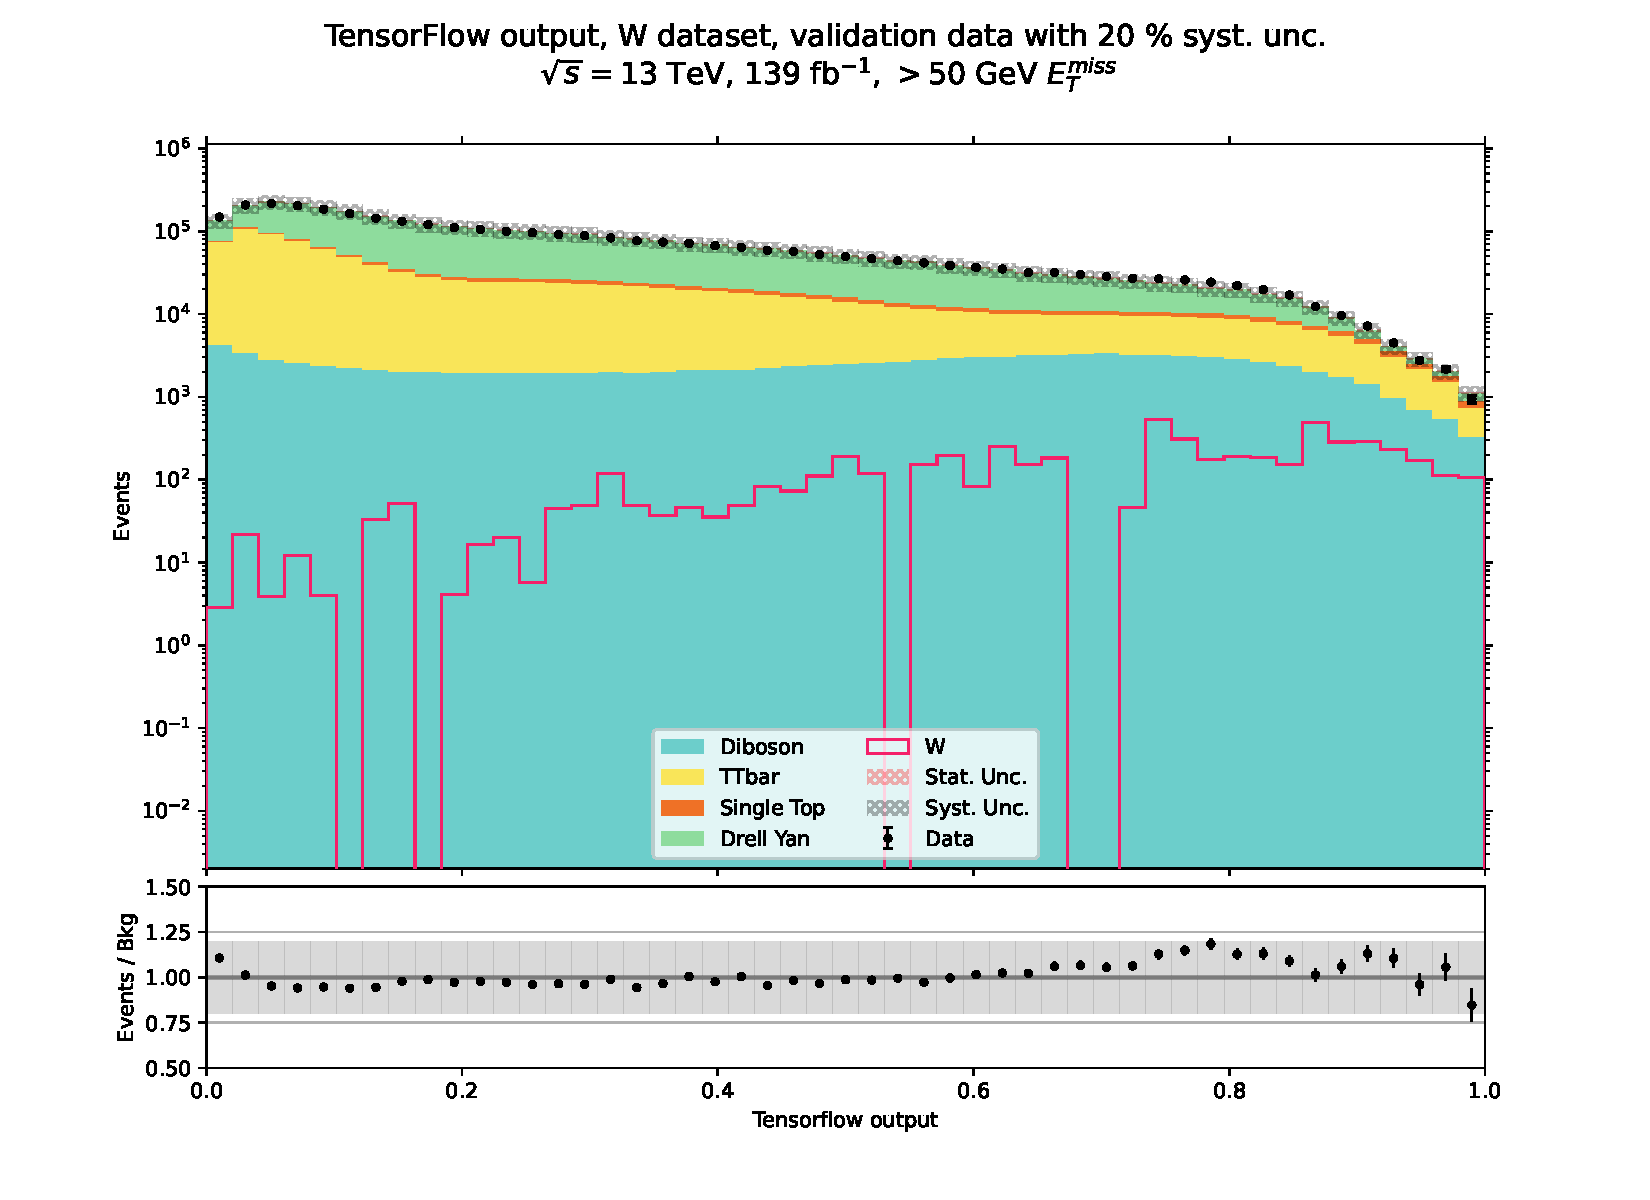
\includegraphics[width=1\textwidth]{Balanced/VAL.pdf}
         \caption{Using ADAM}
      \end{subfigure}
      \begin{subfigure}[b]{0.49\textwidth}
         \centering
         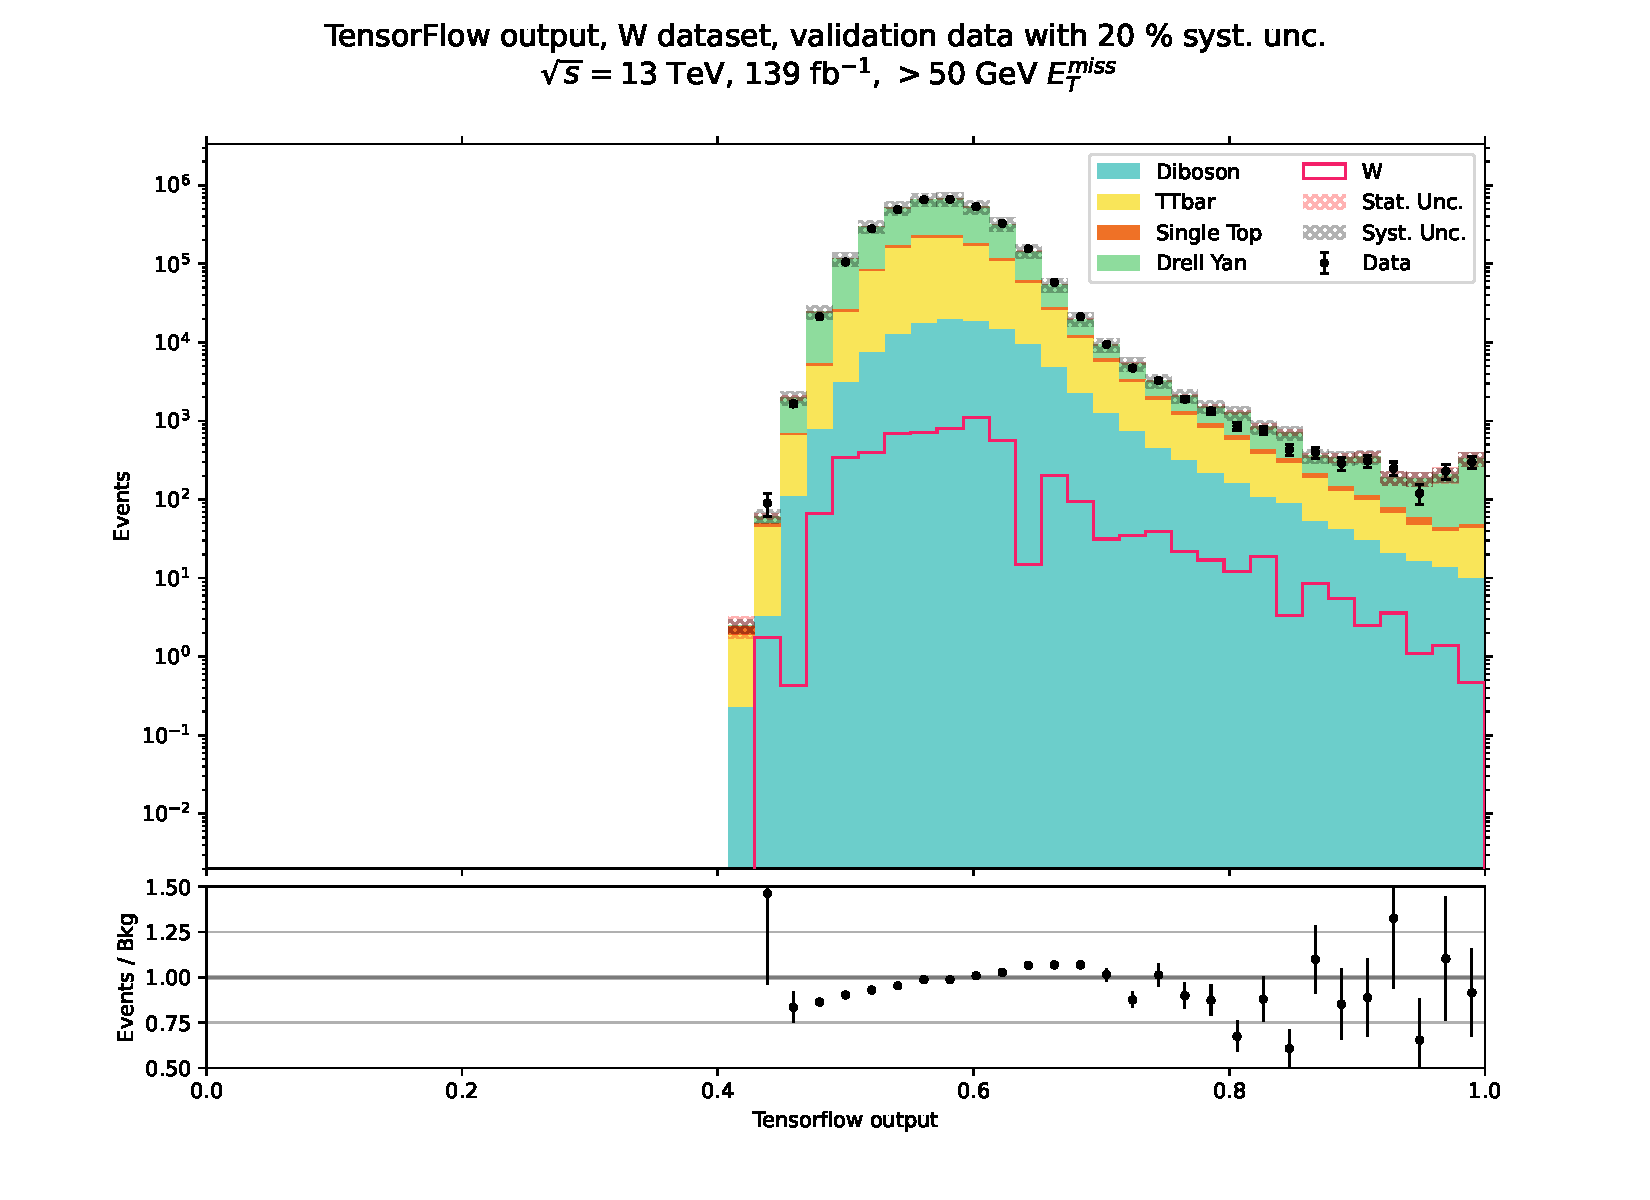
\includegraphics[width=1\textwidth]{SGD/Balanced/VAL.pdf}
         \caption{Using SGD}
      \end{subfigure}
      \caption[Difference between ADAM and SGD optimizer]{Validation plots using SGD and ADAM. 
      This was done using a dataset where the goal was to isloate the $W$ background process from other SM background processes}\label{fig:ADAMvsSGD}
\end{figure}
\\As ADAM is far better at sorting signal from background we will only use this optimizer further. The results for the different weighting methods can be seen in Figure \ref{fig:WVAL}, which shows the 
validation plots and in Figure \ref{fig:WROC} which shows the ROC score. For more Figures showing NN training results see the GitHub repo\footnote{Available here: \href{https://github.com/rubenguevara/Master-Thesis/tree/master/Plots/NeuralNetwork/W}{https://github.com/rubenguevara/Master-Thesis/tree/master/\\Plots/NeuralNetwork/W}}. \\
\begin{figure}[!ht]
	\centering
	\begin{subfigure}[b]{0.49\textwidth}
         \centering
         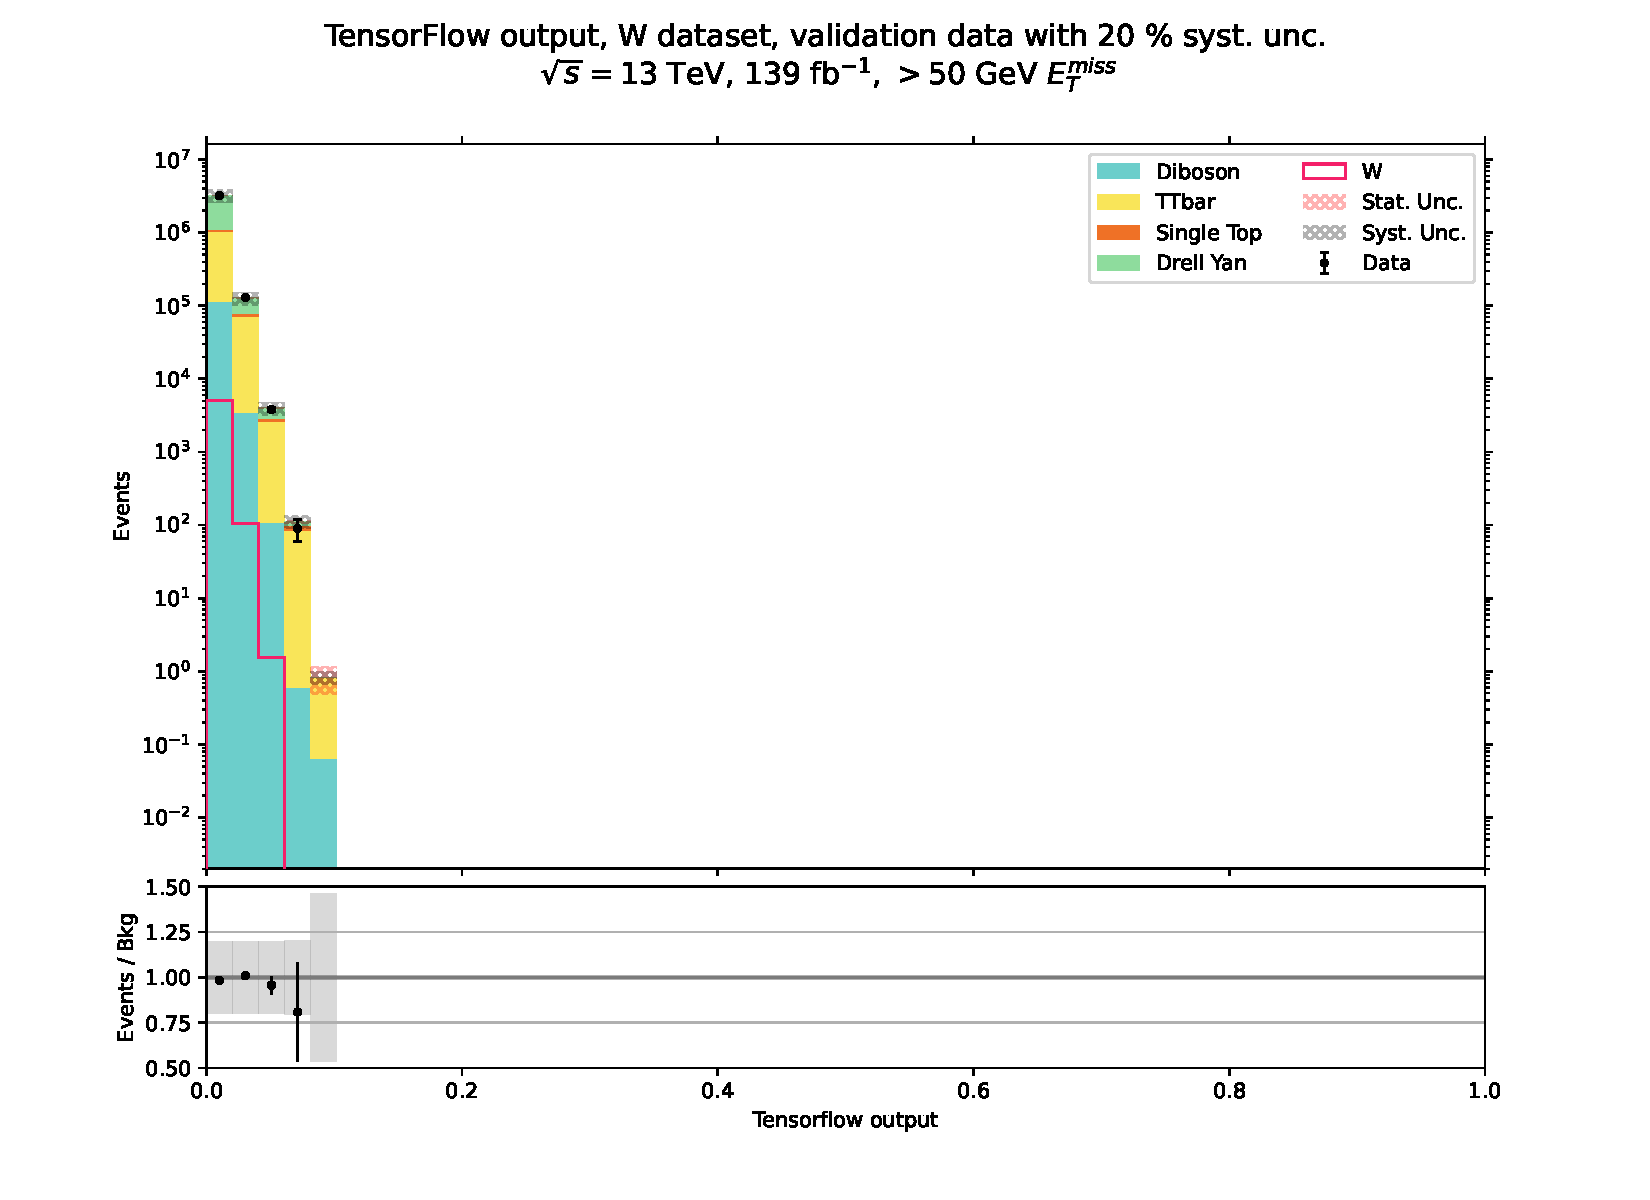
\includegraphics[width=1\textwidth]{Unweighted/VAL.pdf}
         \caption{Using no weights}\label{fig:WVALUW}
      \end{subfigure}
      \hfill
      \begin{subfigure}[b]{0.49\textwidth}
         \centering
         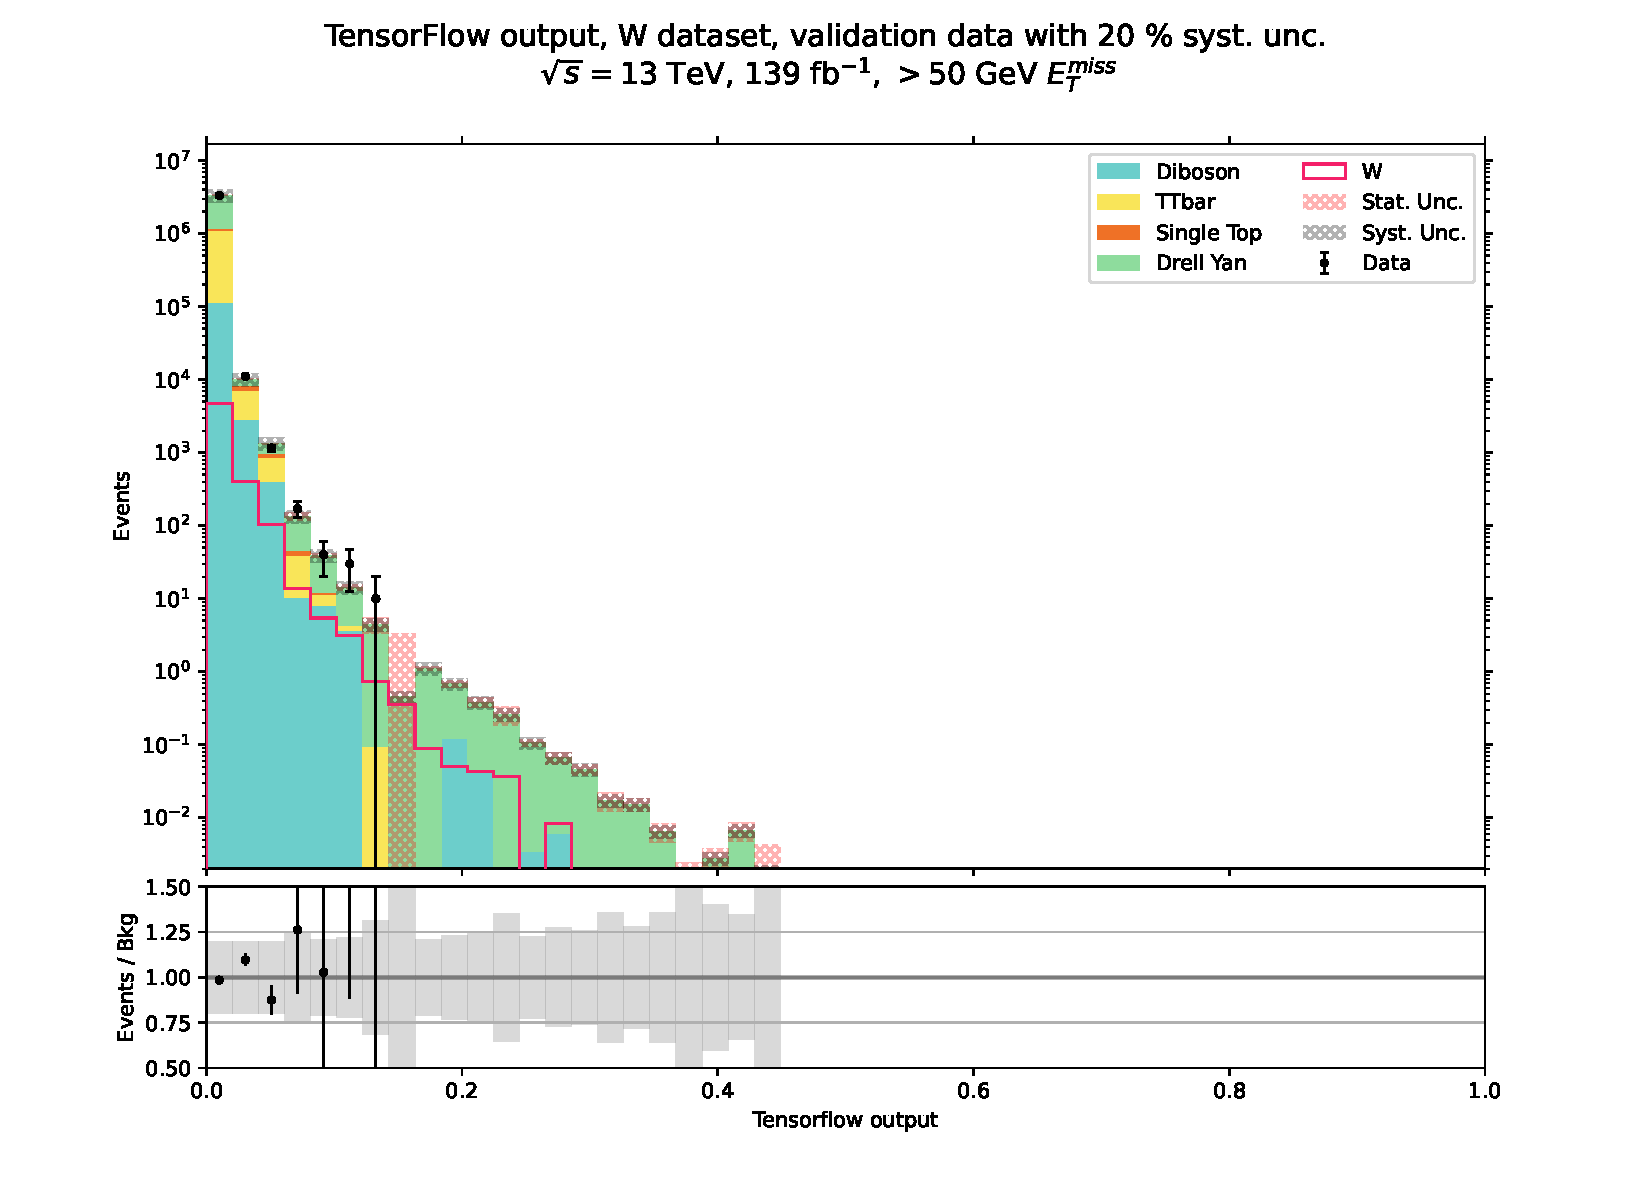
\includegraphics[width=1\textwidth]{Weighted/VAL.pdf}
         \caption{Using re-weighting weights}\label{fig:WVALMC}
      \end{subfigure}
      \begin{subfigure}[b]{0.49\textwidth}
         \centering
         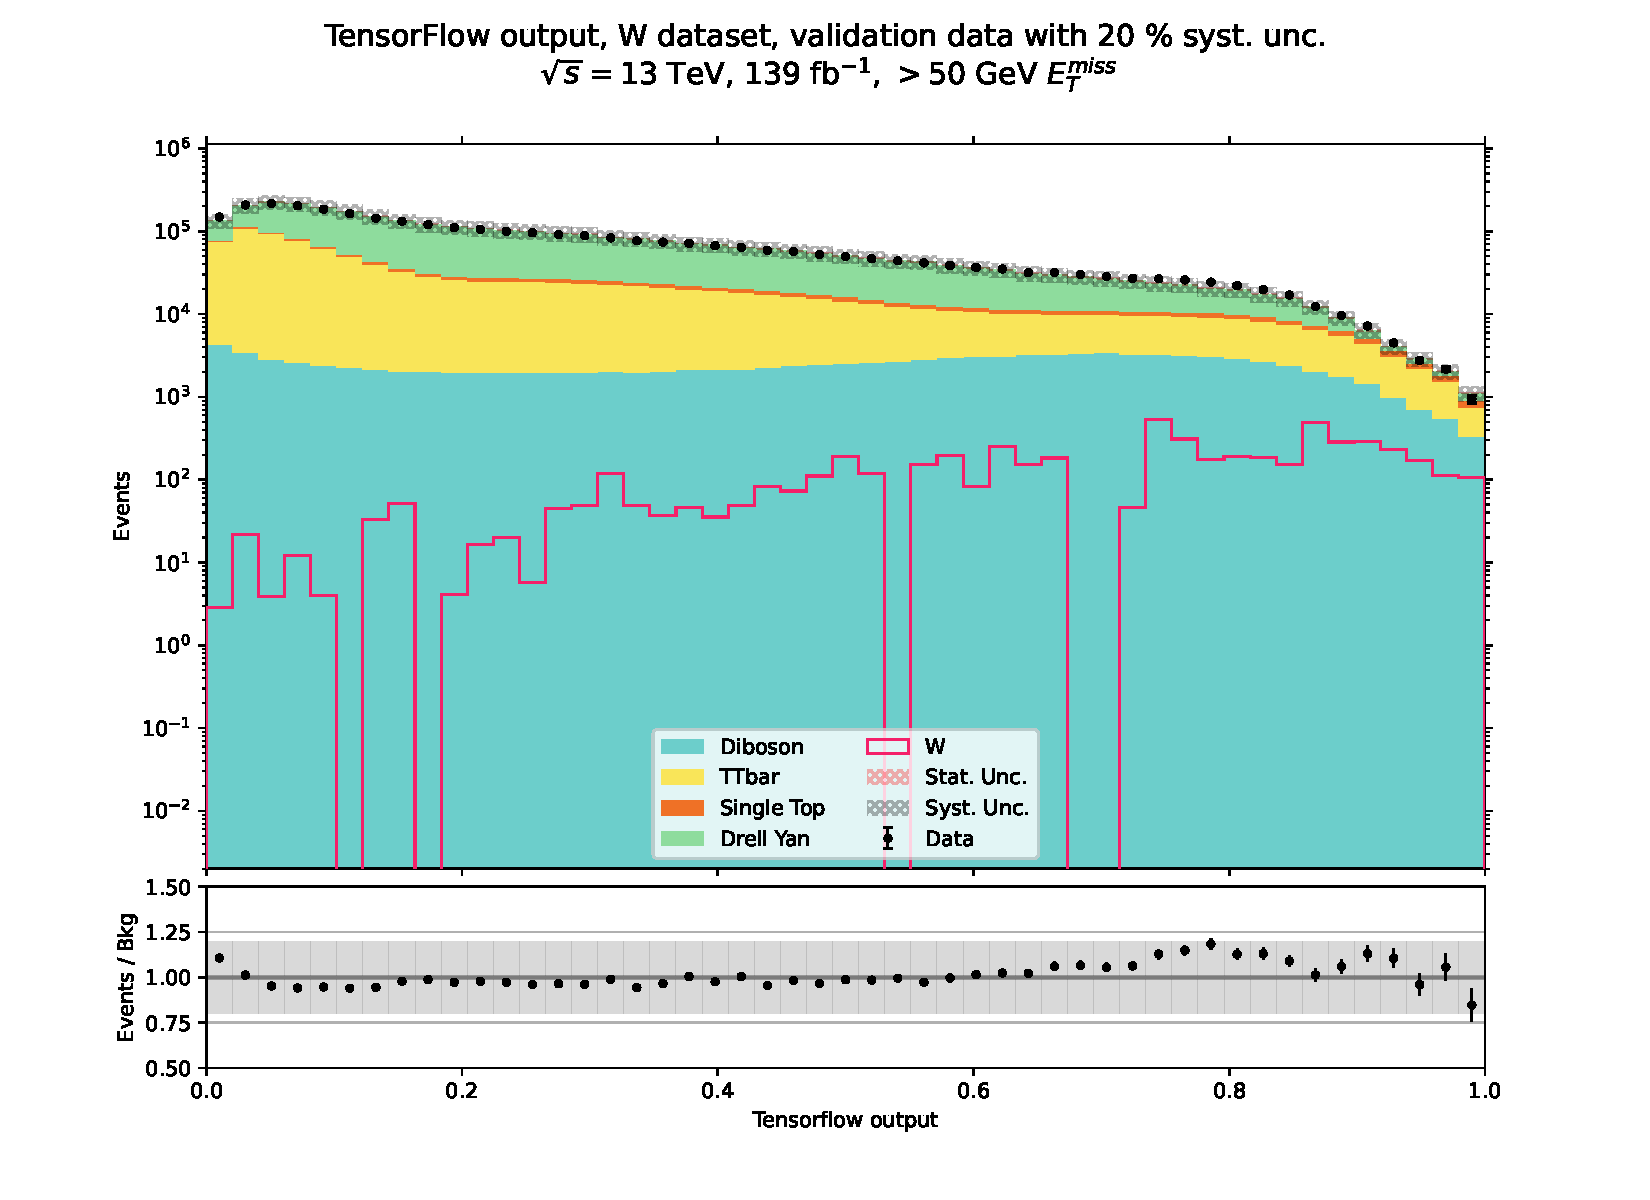
\includegraphics[width=1\textwidth]{Balanced/VAL.pdf}
         \caption{Using $\frac{N_{sig}}{N_{bkg}}$}\label{fig:WVALW}
      \end{subfigure}
      \caption[Validation plots for different balancing methods on NN]{Validation plots of different balancing methods. 
      This was done using a dataset where the goal was to isloate the $W$ background process from other SM background processes}\label{fig:WVAL}
\end{figure}
\begin{figure}[!ht]
	\centering
	\begin{subfigure}[b]{0.49\textwidth}
         \centering
         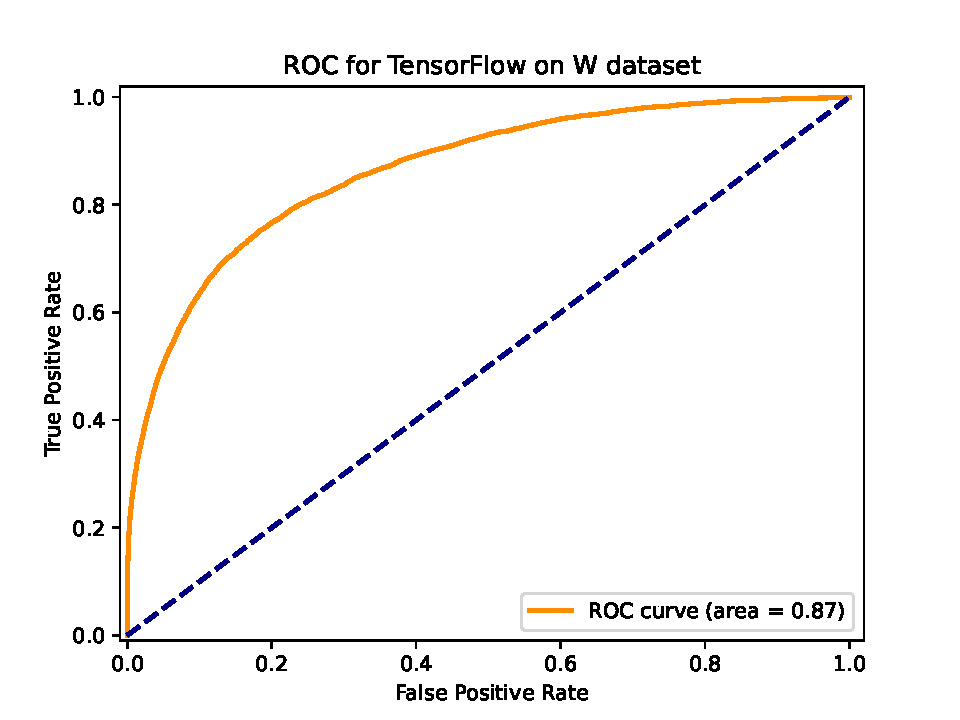
\includegraphics[width=1\textwidth]{Unweighted/ROC.pdf}
         \caption{Using no weights}\label{fig:WROCUW}
      \end{subfigure}
      \hfill
      \begin{subfigure}[b]{0.49\textwidth}
         \centering
         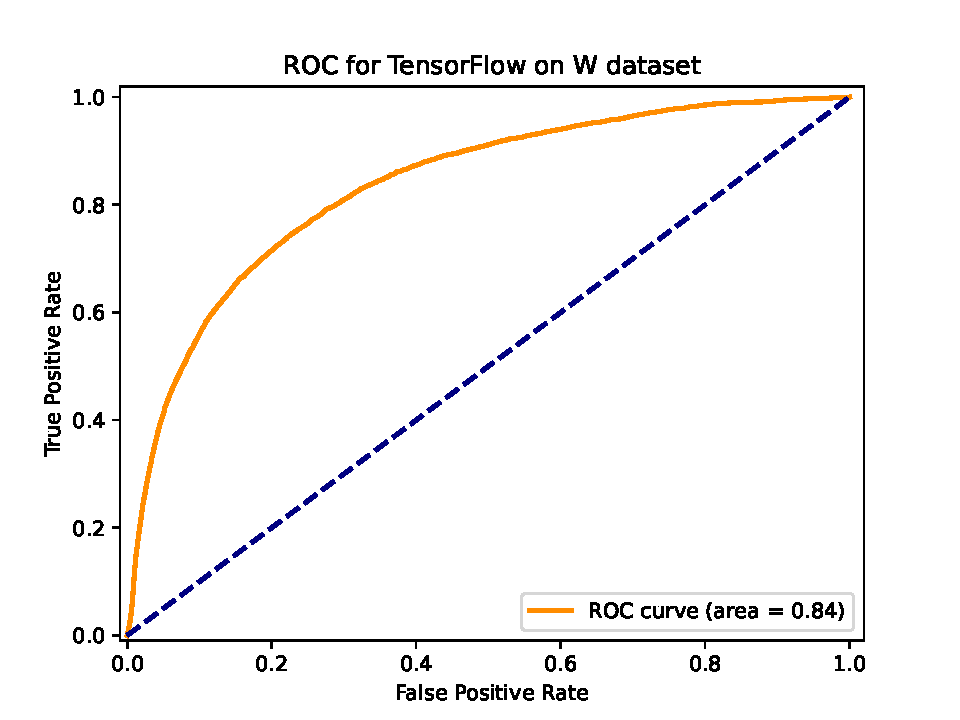
\includegraphics[width=1\textwidth]{Weighted/ROC.pdf}
         \caption{Using re-weighting weights}\label{fig:WROCMC}
      \end{subfigure}
      \begin{subfigure}[b]{0.49\textwidth}
         \centering
         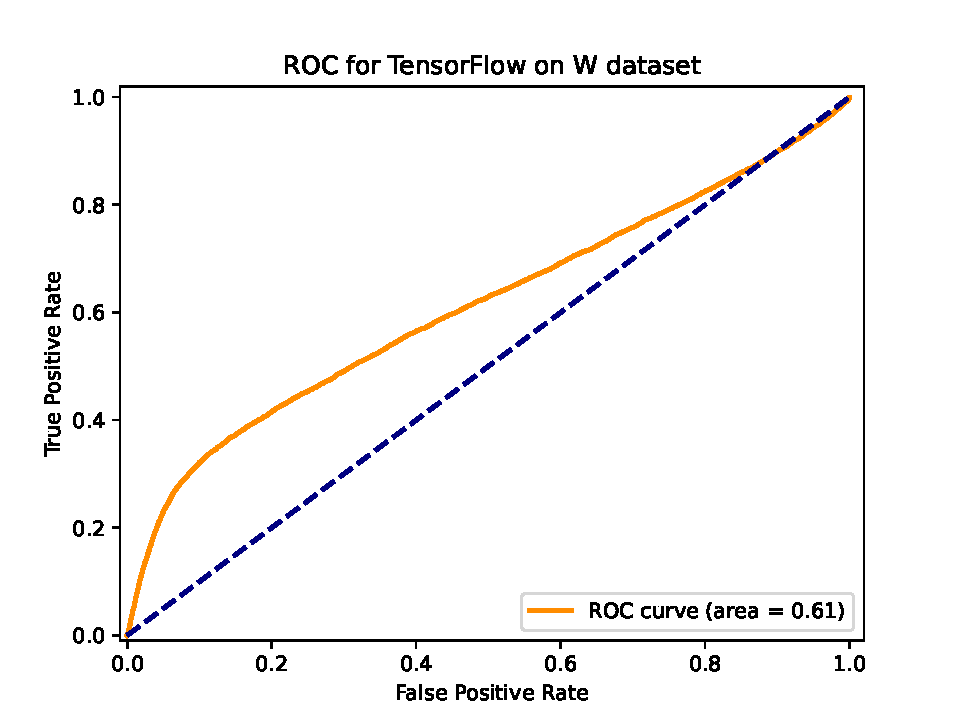
\includegraphics[width=1\textwidth]{Balanced/ROC.pdf}
         \caption{Using $\frac{N_{sig}}{N_{bkg}}$}\label{fig:WROCW}
      \end{subfigure}
      \caption[ROC plots for different balancing methods on NN]{ROC plots of different balancing methods. 
      This was done using a dataset where the goal was to isloate the $W$ background process from other SM background processes}\label{fig:WROC}
\end{figure}
\\From the figures we see that the only way the network does not predict every event to be a background event\footnote{Since the output is the score from 0-1 our network gives every event, where 0 means that the network predicts 0\% chance for an event to be signal} is when we introduce the blancing method. We also see that the AUC increases more as well. Meaning that we must balance our dataset. 
Something else to mention, as to why the network does such a poor job at classifying the W background, is that the network here was not optimized for the search. If we were to conduct a thorough grid search of all hyperparameters it would yield greater results, but as this chapter is for testing methods rather analysing data we will not delve further into it for now,

\clearpage



\subsection{Sample weights to get expected events}\label{sec:samp_wgts_NN_res}
To try the different sample weight methods explained in Chapter \ref{sec:sample_wgts_NN} which include the weights (Chapter \ref{sec:wgts}), we used a dataset consisting of only SM events where the goal was to treat the $W$ channel as signal and try to isolate it from other SM processes. To train we used \verb|Batch_normalization| and 80\% of the SM background events. 
To test we used the remaining 20\% of SM events. The results can be seen in Figure \ref{fig:WVAL_rw}, which shows the validation plots and in Figure \ref{fig:WROC_rw} which shows the ROC score. For more Figures showing NN training results see the GitHub repo\footnote{Available here: \href{https://github.com/rubenguevara/Master-Thesis/tree/master/Plots/NeuralNetwork/W}{https://github.com/rubenguevara/Master-Thesis/tree/master/\\Plots/NeuralNetwork/W}}. 
\begin{figure}[!ht]
	\centering
	\begin{subfigure}[b]{0.49\textwidth}
        \centering
        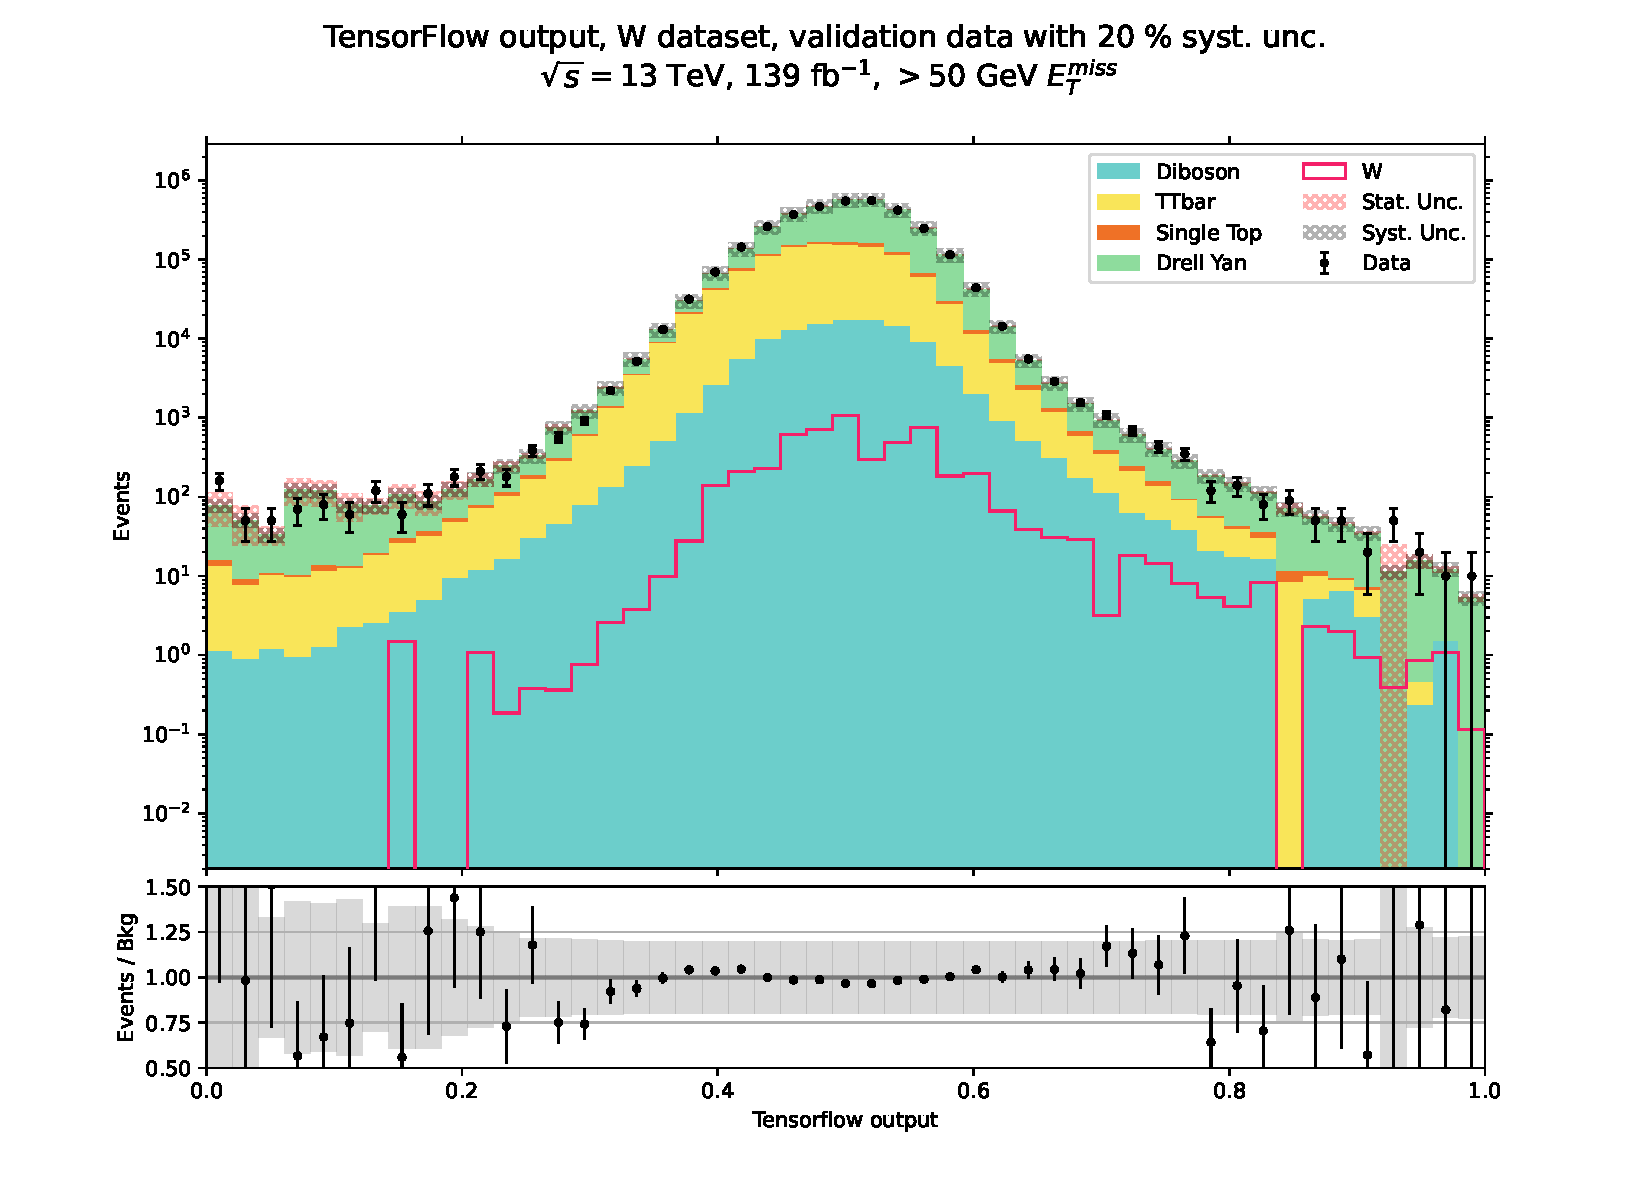
\includegraphics[width=1\textwidth]{bkg_MC/VAL.pdf}
        \caption{Weighing down bkg. wrt. $\frac{N_{sig,MC}}{N_{bkg,MC}}$ }
     \end{subfigure}
     \hfill
     \begin{subfigure}[b]{0.49\textwidth}
        \centering
        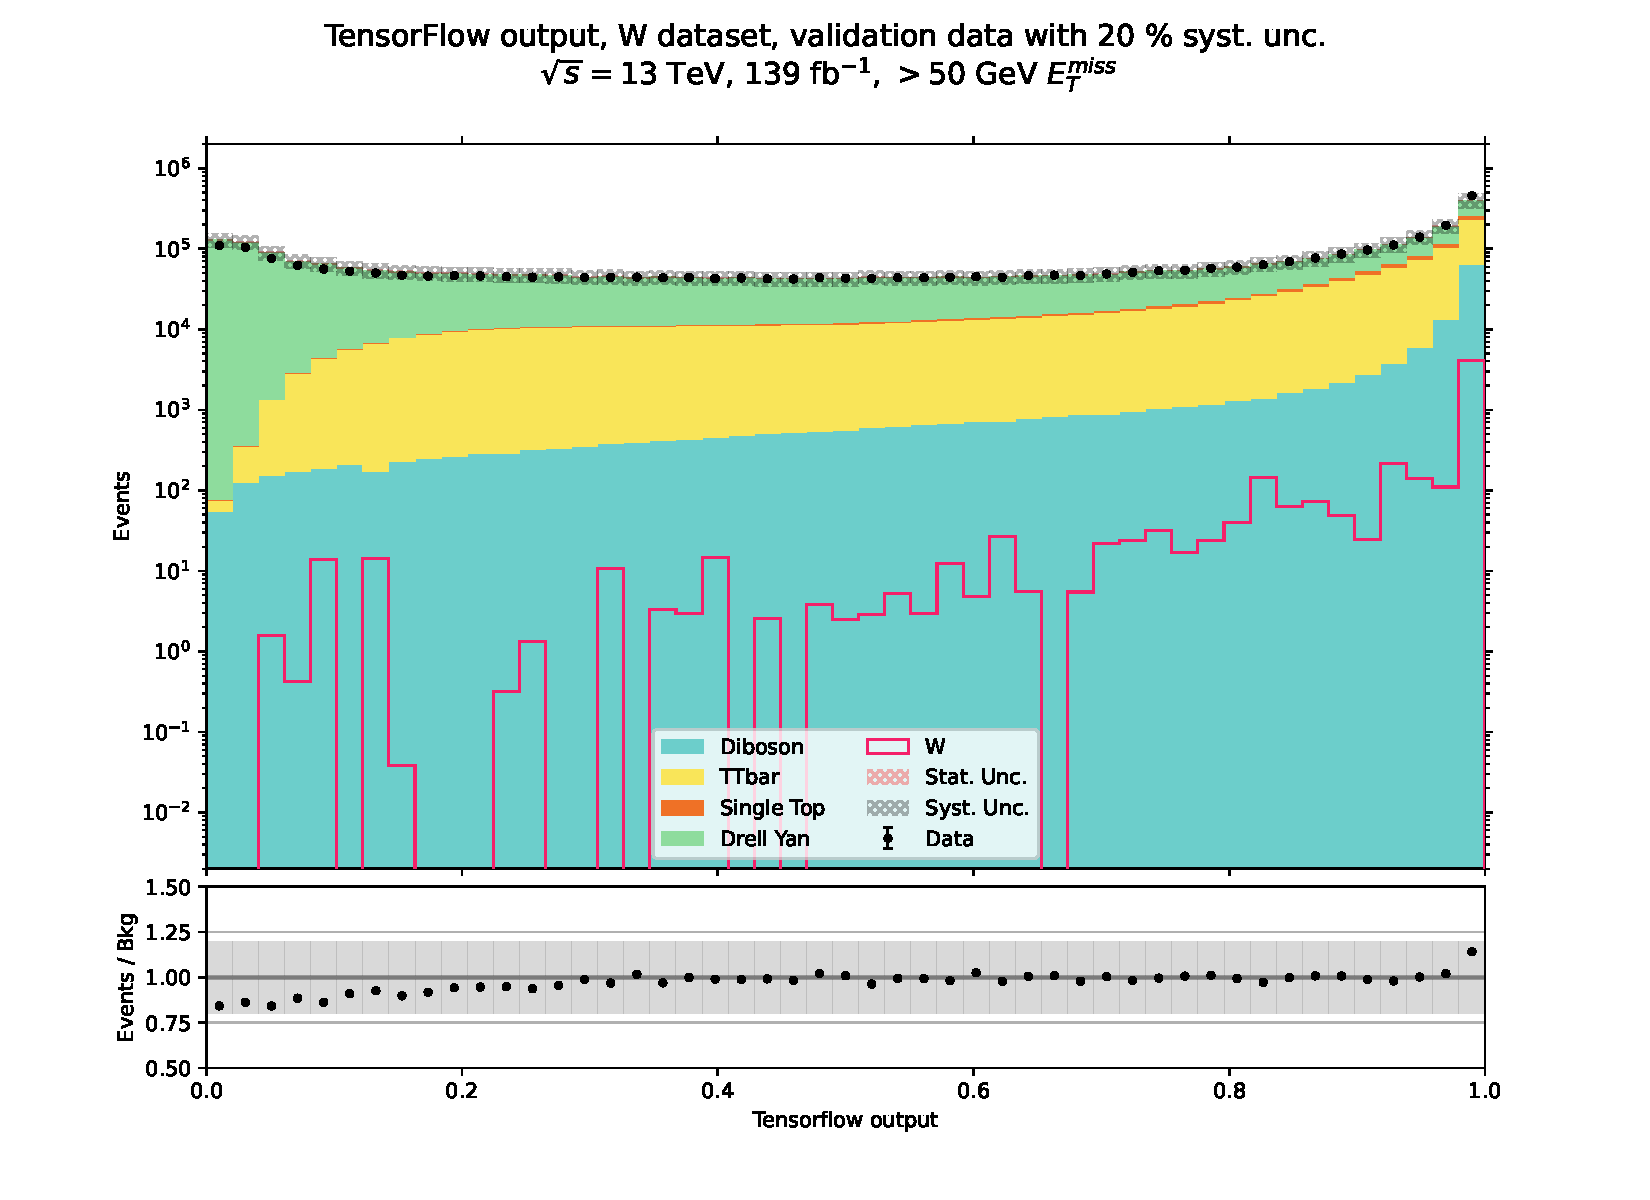
\includegraphics[width=1\textwidth]{sig_MC/VAL.pdf}
        \caption{Weighing up sig. wrt. $\frac{N_{bkg,MC}}{N_{sig,MC}}$}
     \end{subfigure}
     \hfill
     \begin{subfigure}[b]{0.49\textwidth}
          \centering
          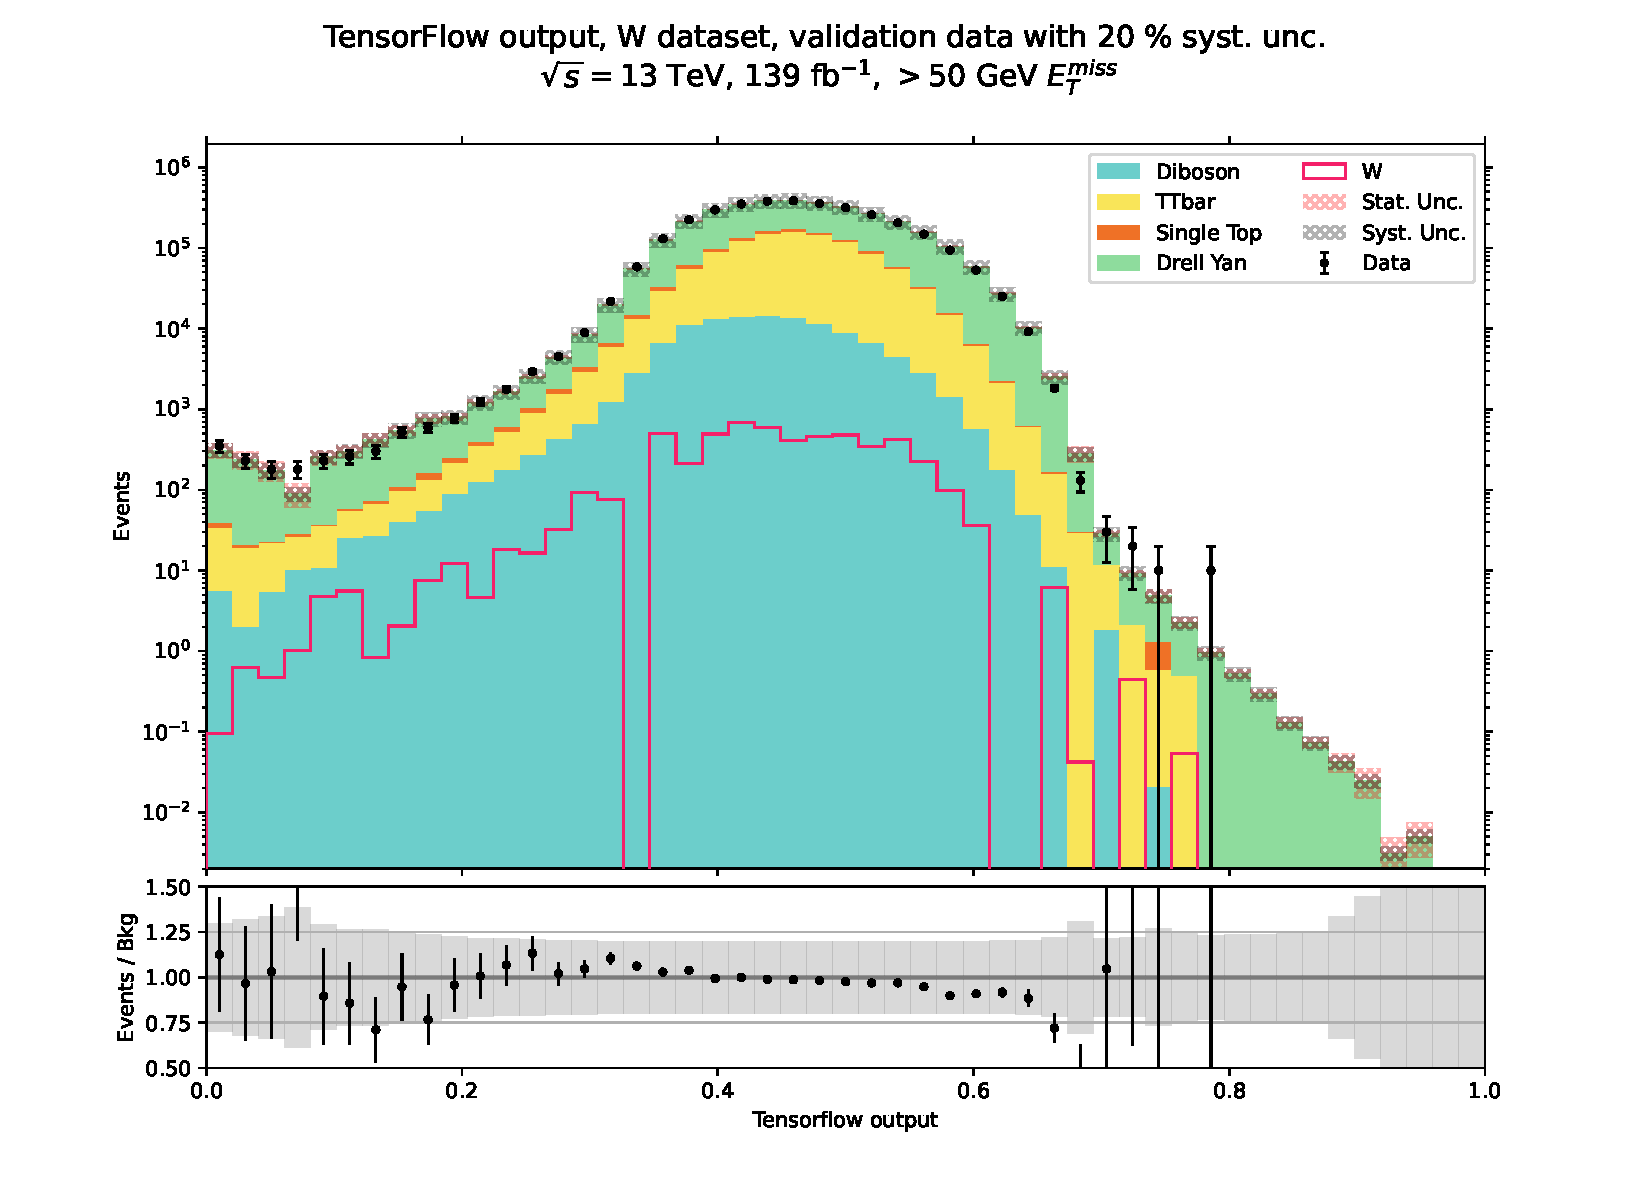
\includegraphics[width=1\textwidth]{bkg_exp/VAL.pdf}
          \caption{Weighing down bkg. wrt. $\frac{N_{sig,MC}}{N_{bkg,exp}}$ }
       \end{subfigure}
       \hfill
       \begin{subfigure}[b]{0.49\textwidth}
          \centering
          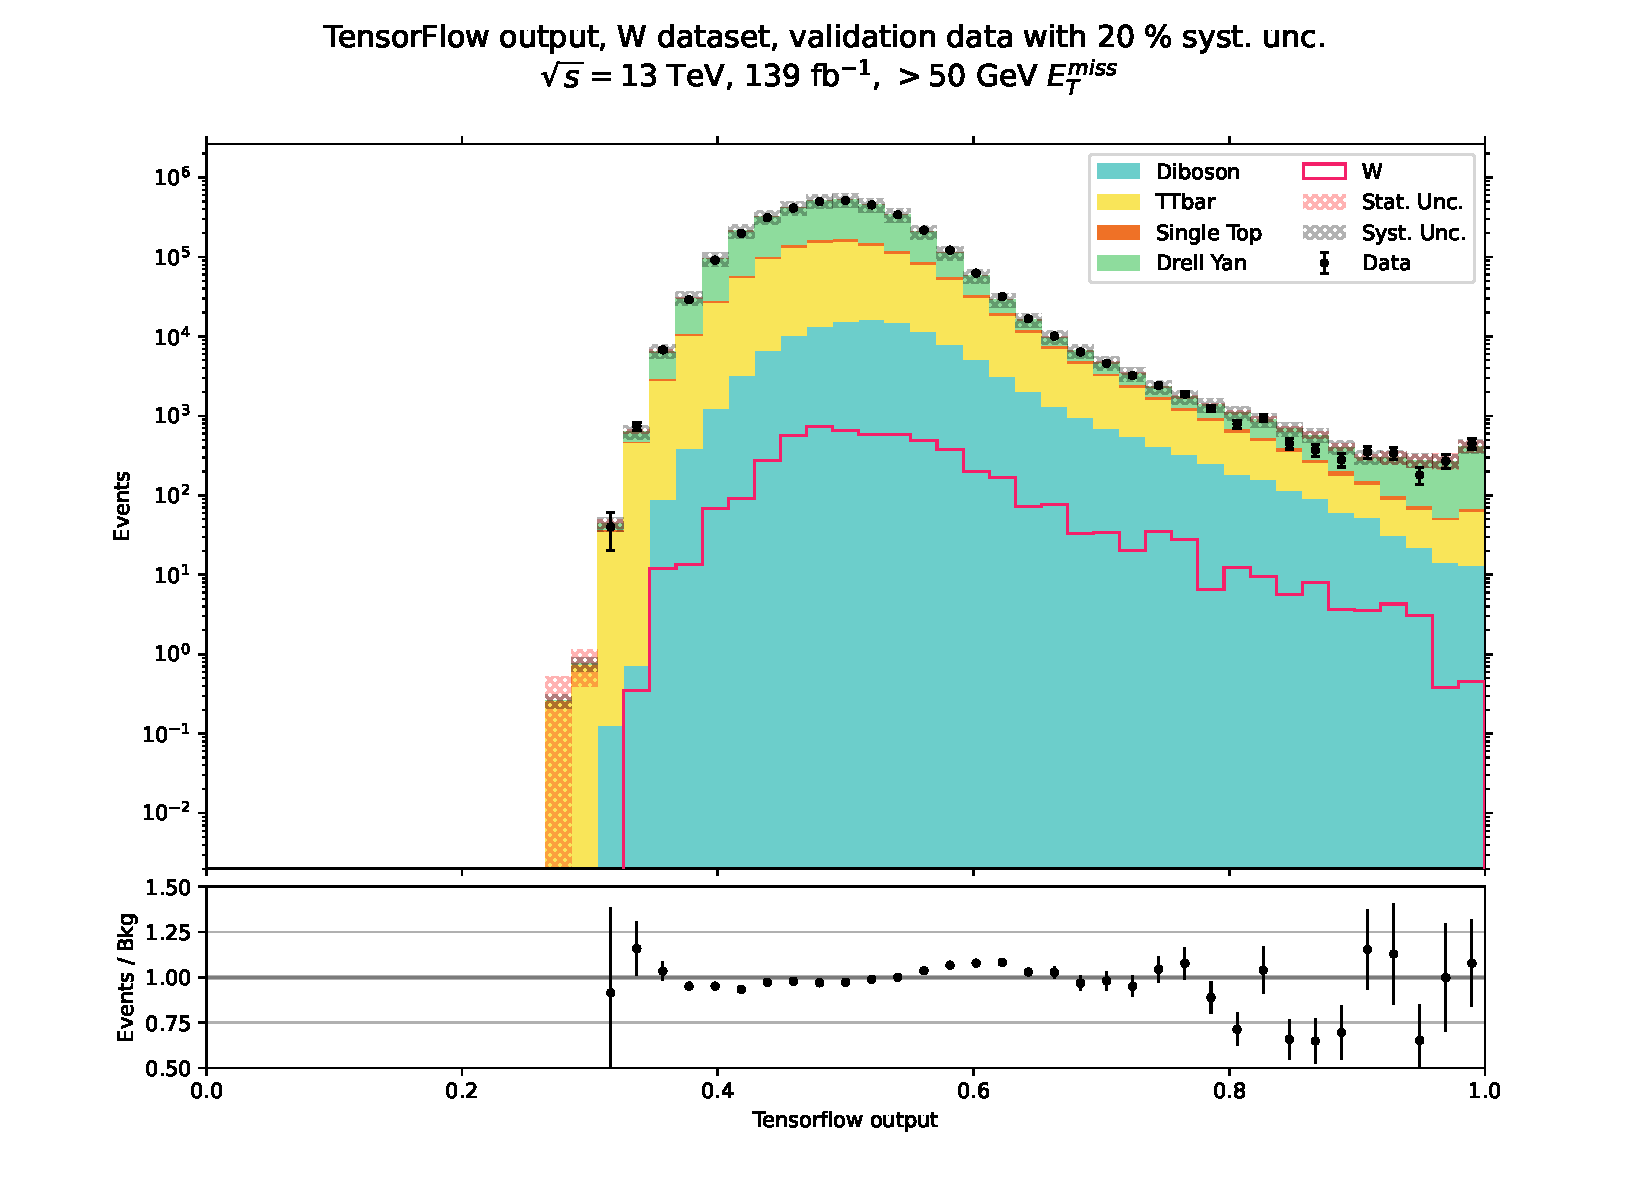
\includegraphics[width=1\textwidth]{sig_exp/VAL.pdf}
          \caption{Weighing up sig. wrt. $\frac{N_{bkg,exp}}{N_{sig,MC}}$}
       \end{subfigure}
     \caption[Validation plots for re-weighting background to expected events on NNs]{Validtion plots of different balancing methods when re-weighint background events to expected events. 
     This was done using a dataset where the goal was to isloate the $W$ background process from other SM background processes} \label{fig:WVAL_rw}
\end{figure}
\begin{figure}[!ht]
	\centering
	\begin{subfigure}[b]{0.49\textwidth}
         \centering
         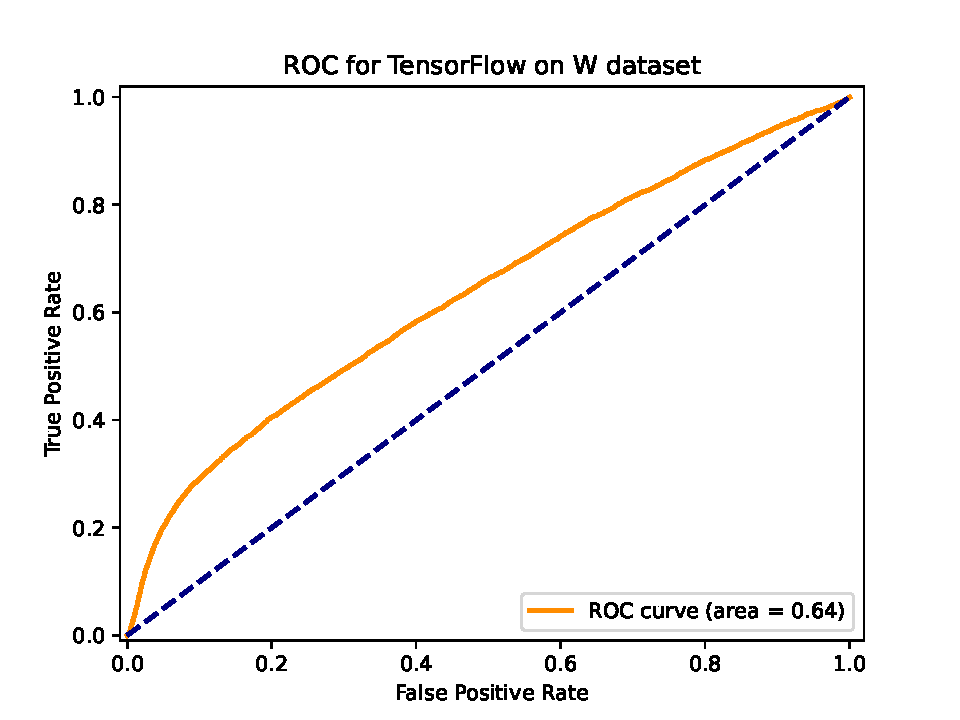
\includegraphics[width=1\textwidth]{bkg_MC/ROC.pdf}
         \caption{Weighing down bkg. wrt. $\frac{N_{sig,MC}}{N_{bkg,MC}}$ }
      \end{subfigure}
      \hfill
      \begin{subfigure}[b]{0.49\textwidth}
         \centering
         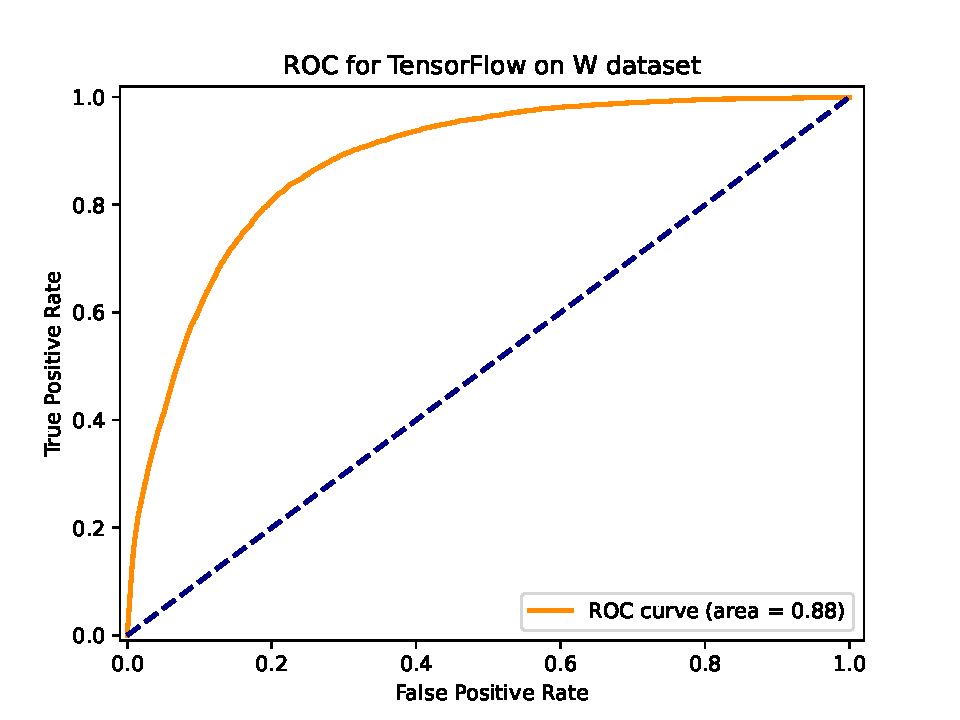
\includegraphics[width=1\textwidth]{sig_MC/ROC.pdf}
         \caption{Weighing up the signal wrt. $\frac{N_{bkg,MC}}{N_{sig,MC}}$}
      \end{subfigure}
      \hfill
      \begin{subfigure}[b]{0.49\textwidth}
            \centering
            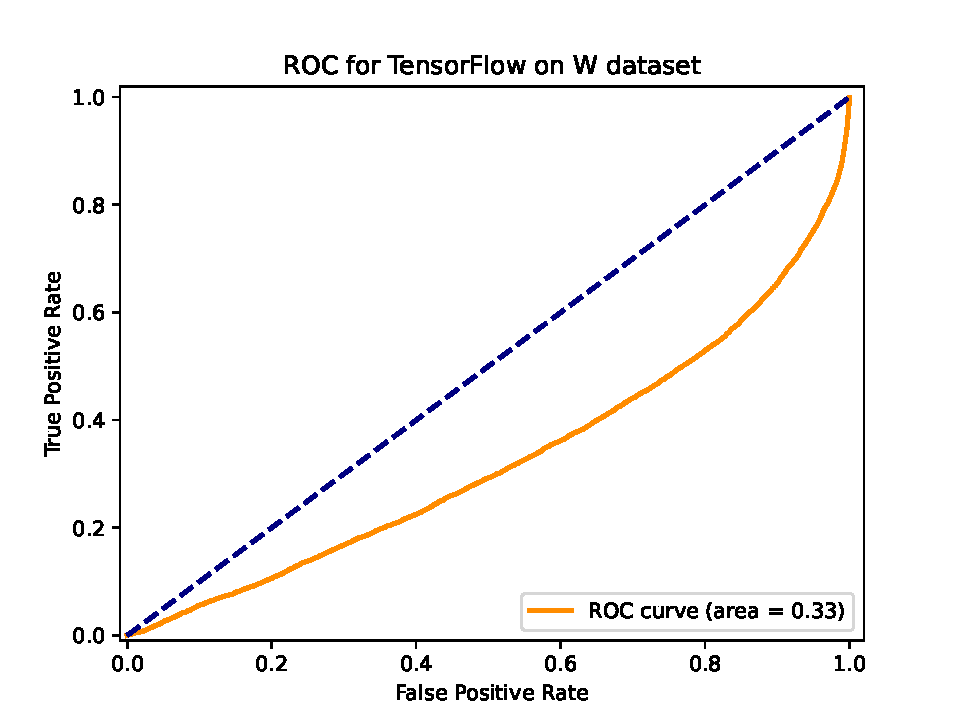
\includegraphics[width=1\textwidth]{bkg_exp/ROC.pdf}
            \caption{Weighing down bkg. wrt. $\frac{N_{sig,MC}}{N_{bkg,exp}}$ }
         \end{subfigure}
         \hfill
         \begin{subfigure}[b]{0.49\textwidth}
            \centering
            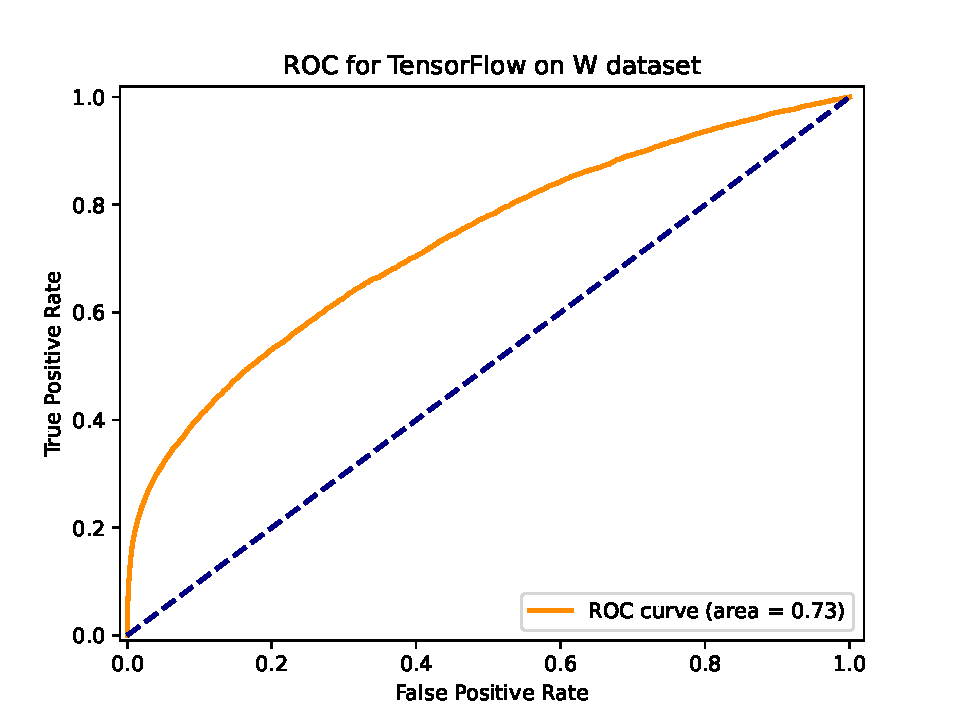
\includegraphics[width=1\textwidth]{sig_exp/ROC.pdf}
            \caption{Weighing up sig. wrt. $\frac{N_{bkg,exp}}{N_{sig,MC}}$}
         \end{subfigure}
      \caption[ROC plots for re-weighting background to expected events on NNs]{ROC plots of different balancing methods when re-weighint background events to expected events. 
      This was done using a dataset where the goal was to isloate the $W$ background process from other SM background processes}\label{fig:WROC_rw}
\end{figure}
\\As we are only re-weighting the background events, we can see from the figures that we get the best results when balancing with respect to the expected number of background events. Which is optimal, as this is what goes into the network. 
Wheter it is better to weigh down the background or weight up the signal is not clear however, from the AUC of the ROC curves it is slightly better to weigh up the signal. To check which gives a higher expected significance however we can look at 
the expected signficance, this is shown in Figure \ref{fig:WSIG}. Here we see that there is a greater expected significance when weighing up the signal events. \\
\begin{figure}[!ht]
	\centering
      \begin{subfigure}[b]{0.49\textwidth}
            \centering
            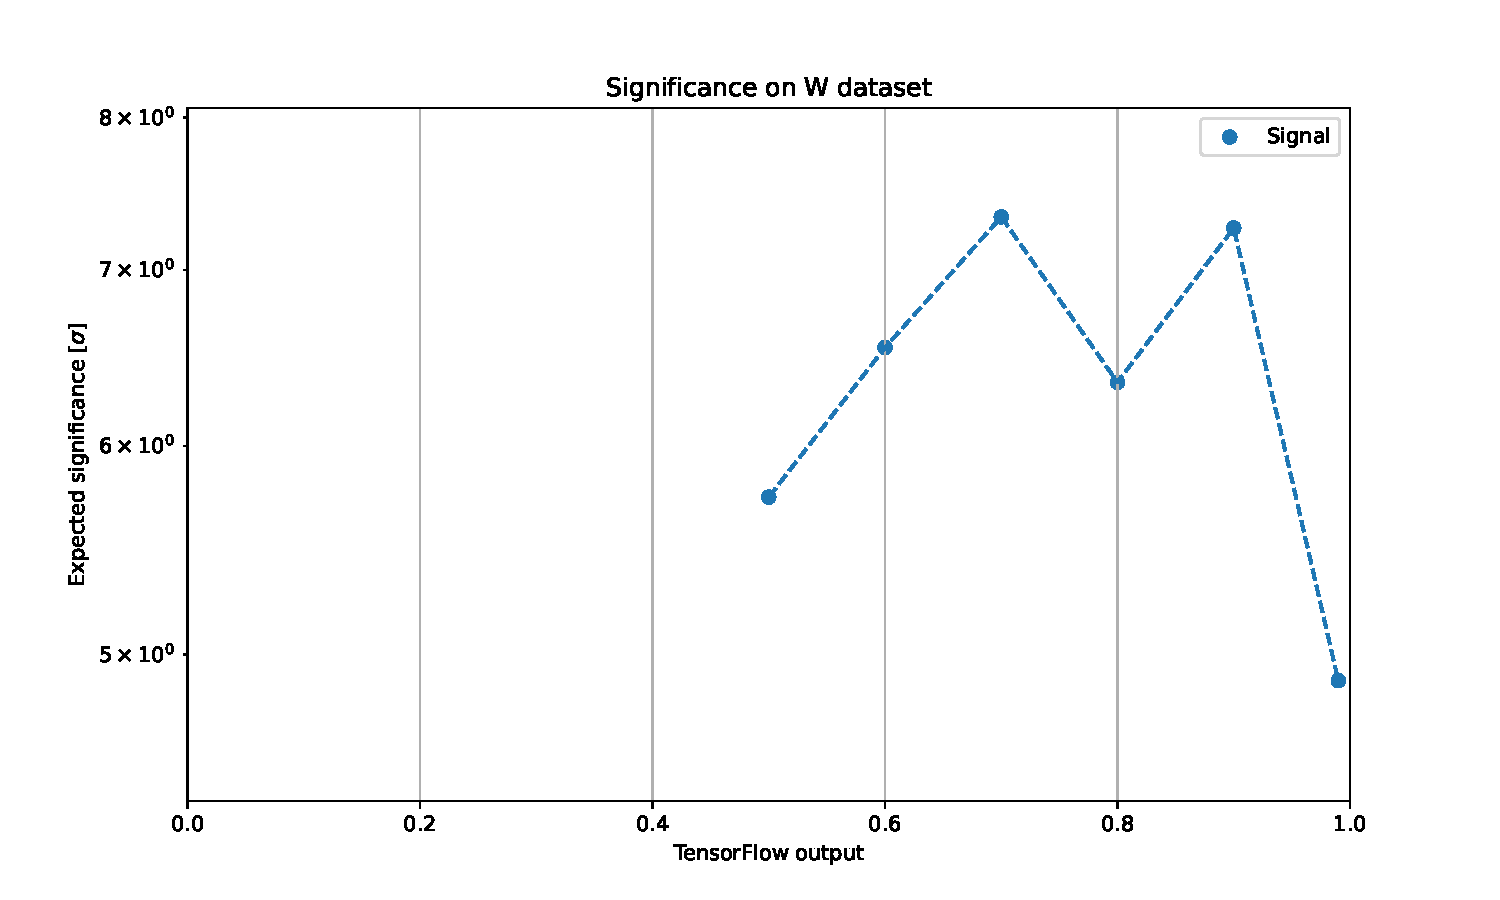
\includegraphics[width=1\textwidth]{bkg_exp/EXP_SIG.pdf}
            \caption{Weighing down bkg. wrt. $\frac{N_{sig,MC}}{N_{bkg,exp}}$ }
         \end{subfigure}
         \hfill
         \begin{subfigure}[b]{0.49\textwidth}
            \centering
            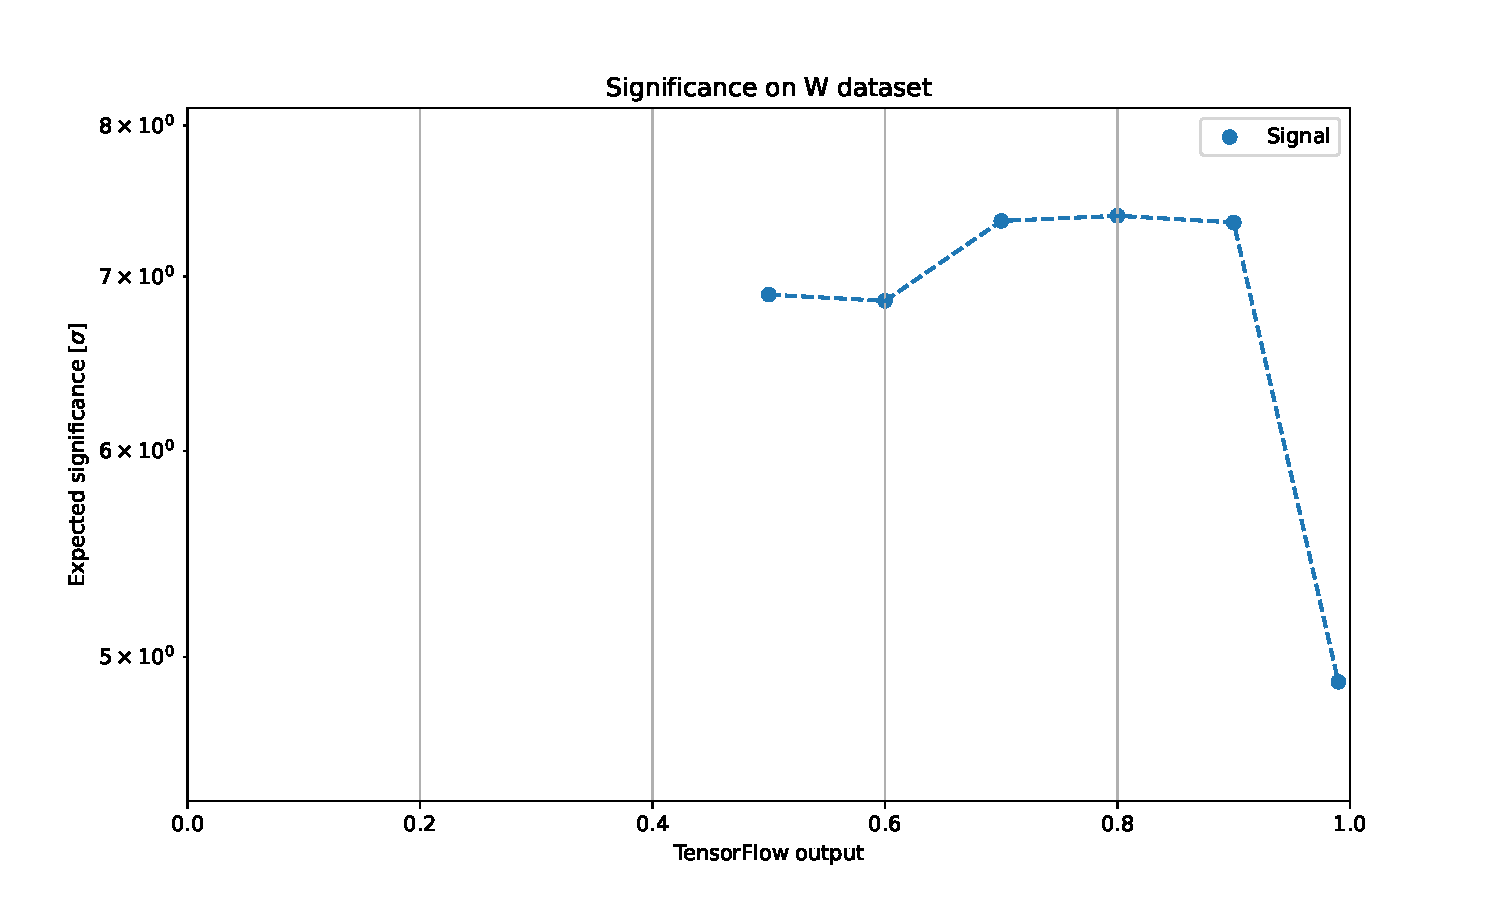
\includegraphics[width=1\textwidth]{sig_exp/EXP_SIG.pdf}
            \caption{Weighing up sig. wrt. $\frac{N_{bkg,exp}}{N_{sig,MC}}$}
         \end{subfigure}
      \caption[Significance plots for re-weighting and balancing W datset on NNs]{Expected significance plots of the best balancing methods when re-weighint background events to expected events. 
      This was done using a dataset where the goal was to isloate the $W$ background process from other SM background processes}\label{fig:WSIG}
\end{figure}
\\As a last note for the testing of these methods, the networks, while still getting over 5$\sigma$ expected significance (without errors) on the $W$ chanel, do not have the best distribution on the validation plots. The reason for this might be because 
we did not optimize the networks we tested, but rather used the same network for test. 
\clearpage


\subsection{Padding of data}\label{sec:padding_NN_res}
For the padding problem. We will as explained in Chapter \ref{sec:padding_NN} try the new variables presented in Table \ref{tab:padding_variables}. The other method we tried was to remove the features with jagged arrays, that means the $p_T, \eta, \phi$ of the three most energetic jets, as well as the invariant mass of the two most energetic ones, $m_{jj}$.
e trained a network using 80\% of the whole SM background events as well as 80\% of all the Z' DH HDS samples. As sample weights we used the best method from the previous section, which was to re-weight every background event and balance the dataset by weighing up all signal events by the ratio of expected number of background events over signal MC events, $\frac{N_{bkg,exp}}{N_{sig,MC}}$. 
As the best normaliazation method was \verb|Batch_normalization|, this method was used here. We also utilized the ADAM optimizer instead of SGD.\\
\\As changing features technically changes the whole dataset, then to get the best results as possile we went through a full grid search following the steps in Chapter \ref{sec:NNgriddy} for both networks. The result for the hyperparameters that gave the highest significance can be seen in Figure \ref{fig:pad_griddy}.
\graphicspath{{../../../Plots/NeuralNetwork/Padding/}}
\begin{figure}[!ht]
	\centering
	\begin{subfigure}[b]{0.49\textwidth}
      \centering
      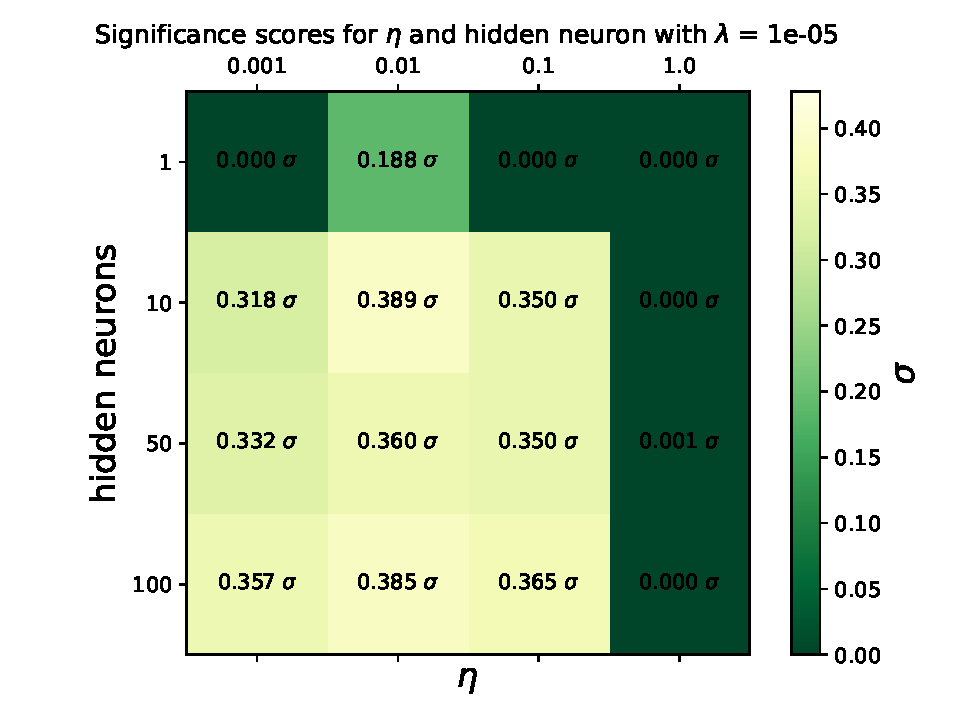
\includegraphics[width=1\textwidth]{New_pad/GRID/Significance_ne.pdf}
      % \includegraphics[width=1\textwidth]{New_pad/GRID/AUC/Testing_nl.pdf}
      \caption{When including new features}
   \end{subfigure}
   \hfill
	\begin{subfigure}[b]{0.49\textwidth}
      \centering
      \includegraphics[width=1\textwidth]{No_pad/GRID/Significance_ne.pdf}
      % \includegraphics[width=1\textwidth]{No_pad/GRID/AUC/Testing_nl.pdf}
      \caption{When dropping features}
   \end{subfigure}
   \caption[Grid search result for pad testing on NN]{Grid search result for pad testing on NN.  This is training a dataset with 80\% of all Z' DH HDS events.}\label{fig:pad_griddy}
\end{figure}
\\This means that the best hyperparemeters when using the new featues are: \verb|n_neuron = 100,| \verb|eta = 1,| \verb|lamda = 1e-3|, and when removing features are: \verb|n_neuron = 1,| \verb|eta = 1,| \verb|lamda = 1e-4|. The loss, AUC and binary accuracy over epochs for the best networks can be seen in Figure \ref{fig:NN_stats_pad} and Figure \ref{fig:NN_stats_no_pad}.
\begin{figure}[!ht]
	\centering
	\begin{subfigure}[b]{0.49\textwidth}
      \centering
      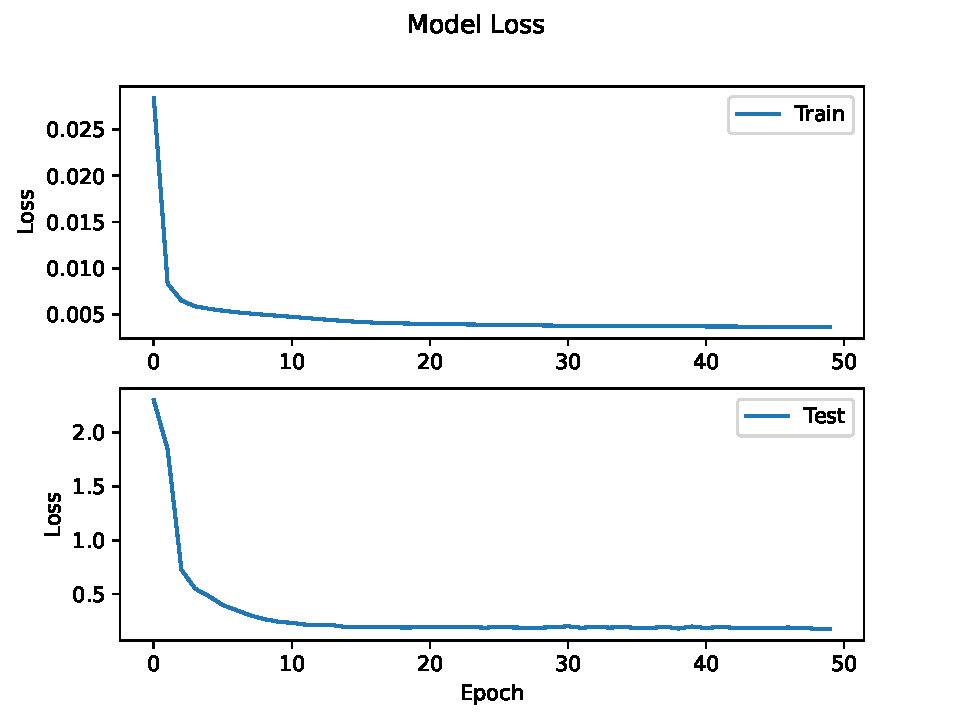
\includegraphics[width=1\textwidth]{New_pad/Loss.pdf}
   \end{subfigure}
   \hfill
	\begin{subfigure}[b]{0.49\textwidth}
      \centering
      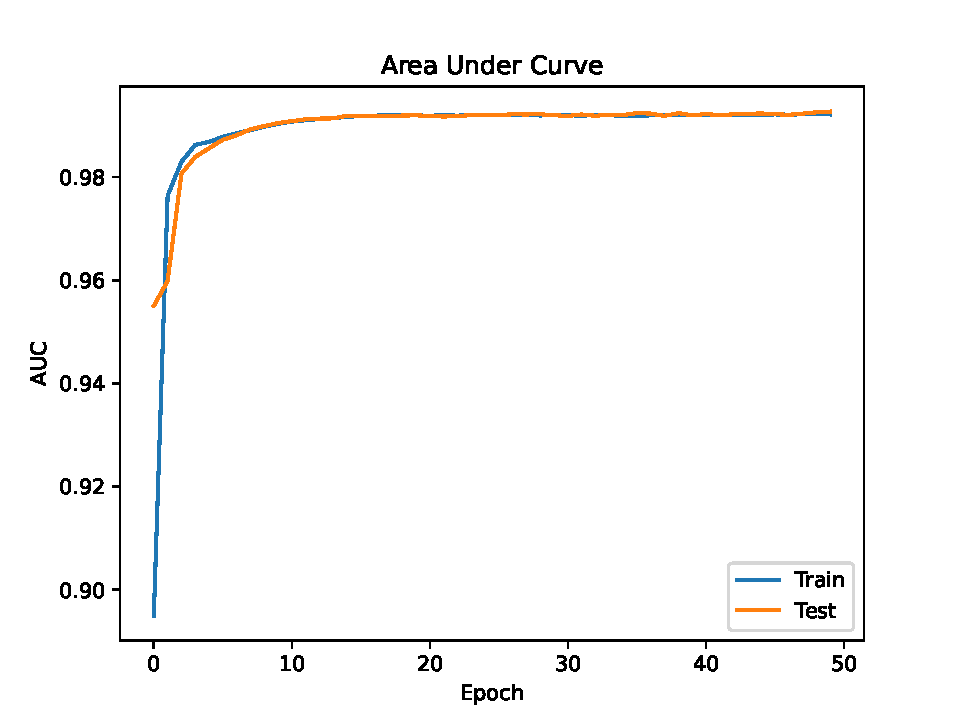
\includegraphics[width=1\textwidth]{New_pad/AUC.pdf}
   \end{subfigure}
   \hfill
	\begin{subfigure}[b]{0.49\textwidth}
      \centering
      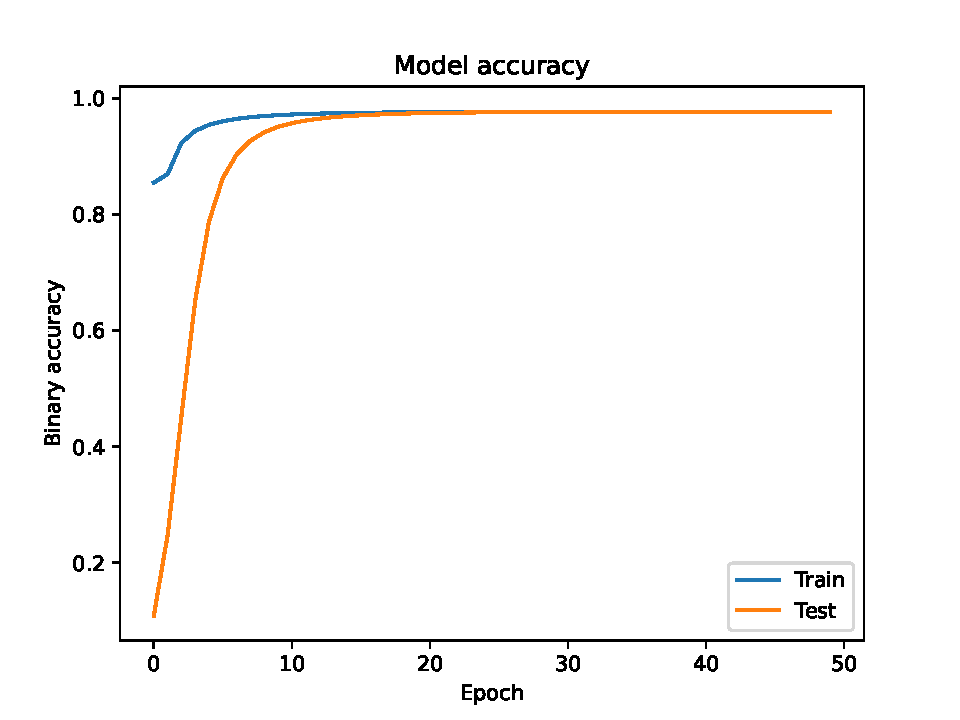
\includegraphics[width=1\textwidth]{New_pad/Binary_accuracy.pdf}
   \end{subfigure}
   \caption[NN parameters after 50 epochs with new features]{NN parameters after 50 epochs with new features.  This is training a dataset with 80\% of all Z' DH HDS events.}\label{fig:NN_stats_pad}
\end{figure}
\begin{figure}[!ht]
	\centering
	\begin{subfigure}[b]{0.49\textwidth}
      \centering
      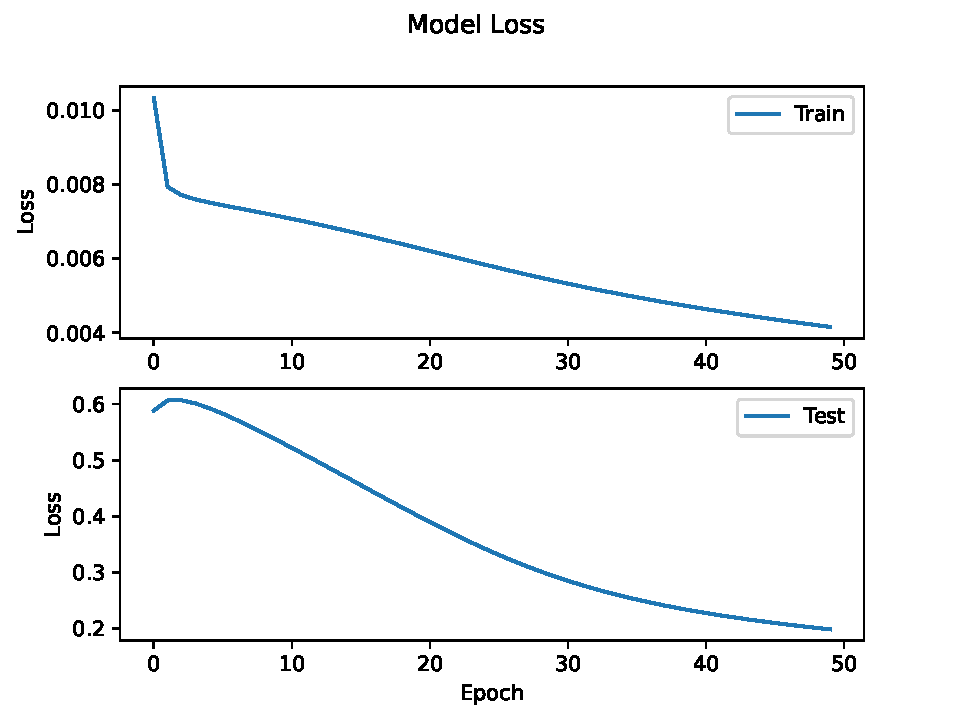
\includegraphics[width=1\textwidth]{No_pad/Loss.pdf}
   \end{subfigure}
   \hfill
	\begin{subfigure}[b]{0.49\textwidth}
      \centering
      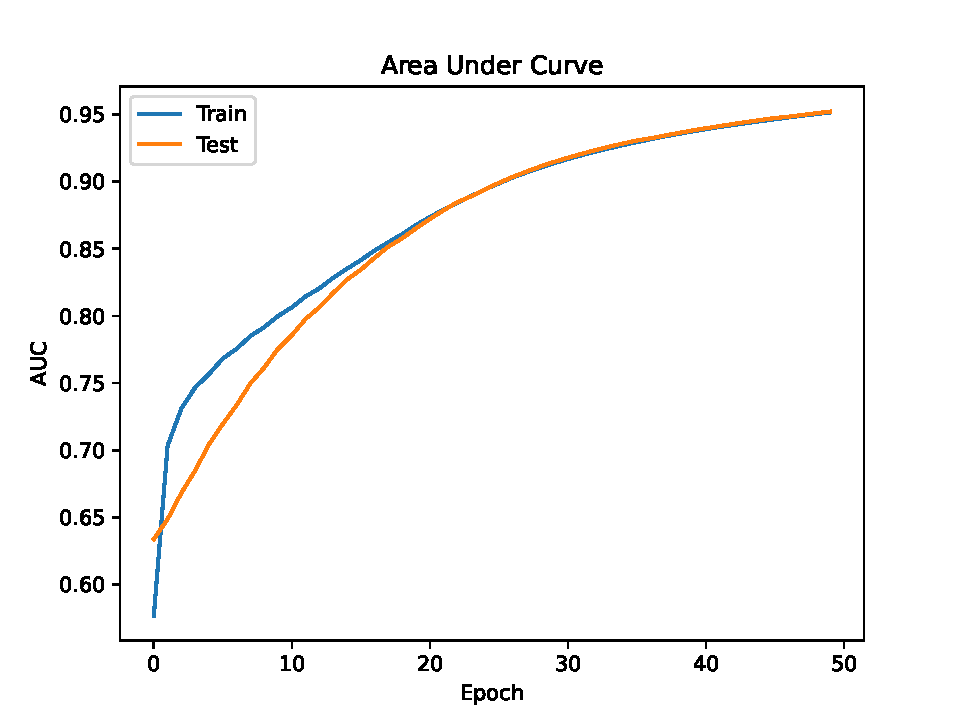
\includegraphics[width=1\textwidth]{No_pad/AUC.pdf}
   \end{subfigure}
   \hfill
	\begin{subfigure}[b]{0.49\textwidth}
      \centering
      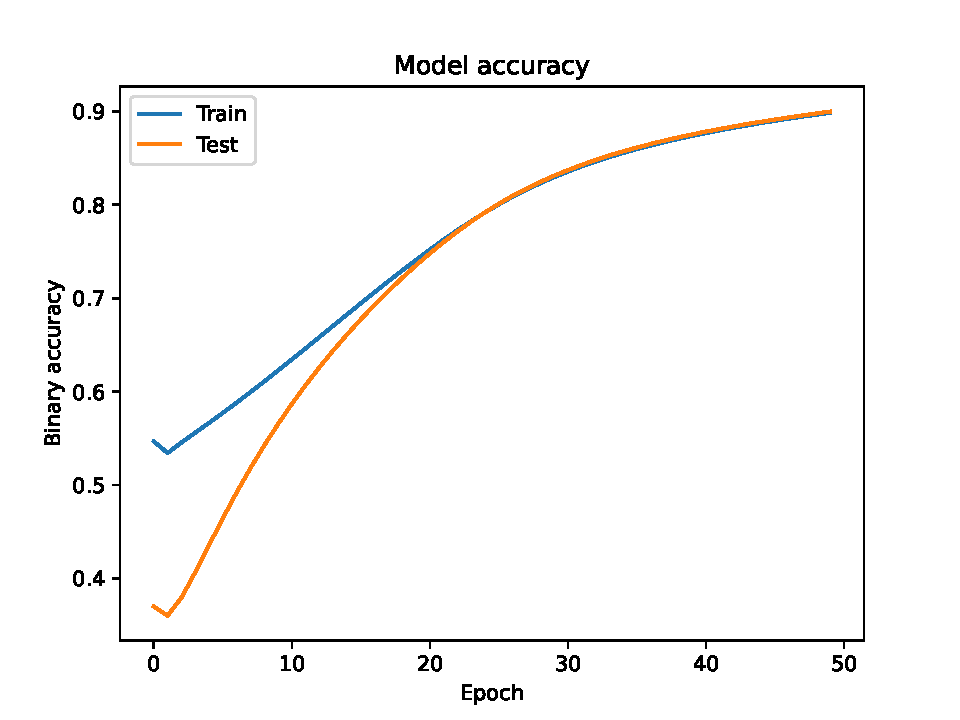
\includegraphics[width=1\textwidth]{No_pad/Binary_accuracy.pdf}
   \end{subfigure}
   \caption[NN parameters after 50 epochs when dropping features]{NN parameters after 50 epochs when dropping features.  This is training a dataset with 80\% of all Z' DH HDS events.}\label{fig:NN_stats_no_pad}
\end{figure}
\\We tested on the remaining 20\% of the SM background events, as well as 20\% of Z' DH HDS events where $m_{Z'} =130$ GeV. The ROC scores for each network can be seen in Figure \ref{fig:NN_pad_ROC}. The validation plots can be seen in Figure \ref{fig:NN_pad_VAL}
\begin{figure}[!ht]
	\centering
	\begin{subfigure}[b]{0.49\textwidth}
      \centering
      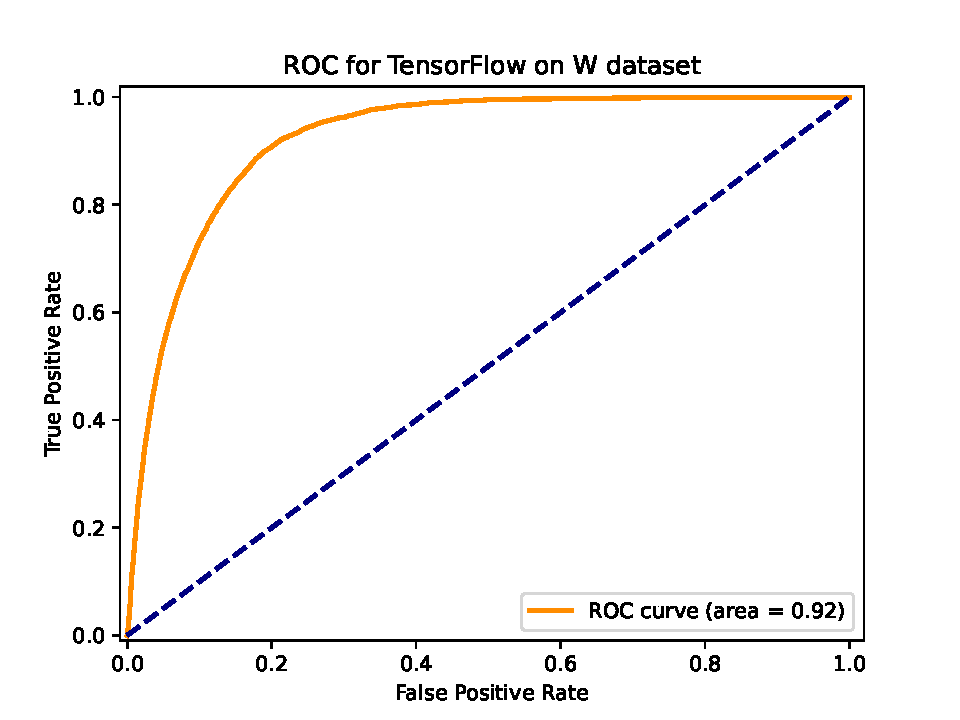
\includegraphics[width=1\textwidth]{New_pad/ROC.pdf}
      \caption{When including new features}
   \end{subfigure}
   \hfill
	\begin{subfigure}[b]{0.49\textwidth}
      \centering
      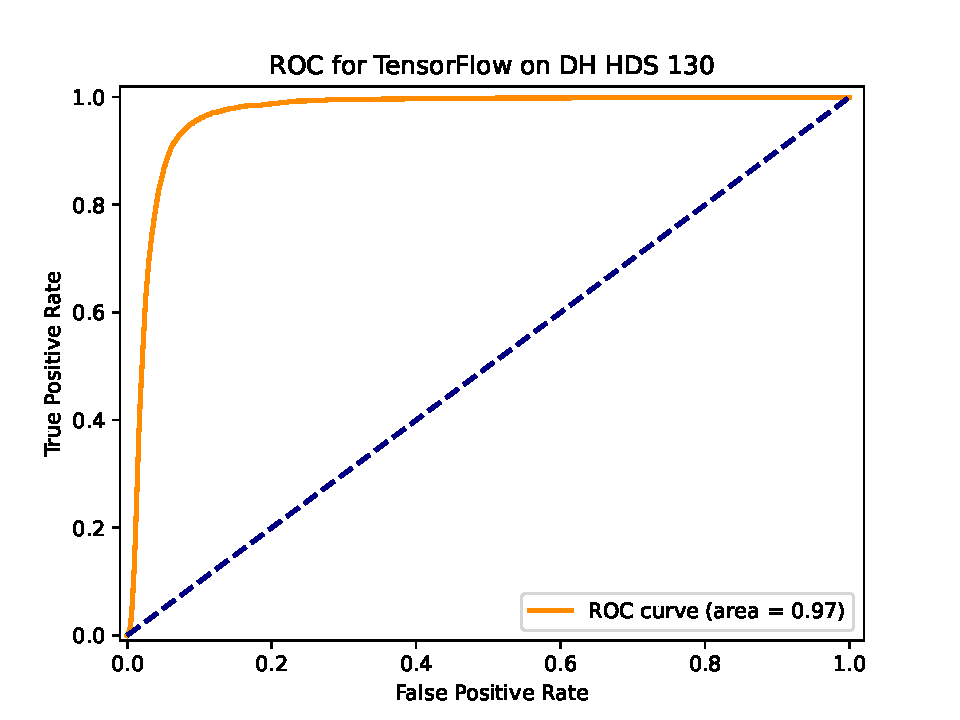
\includegraphics[width=1\textwidth]{No_pad/ROC.pdf}
      \caption{When dropping features}
   \end{subfigure}
   \caption[ROC plots for both padding methods]{ROC plots for both padding methods.  This is testing a dataset with 20\% of the Z' DH HDS $m_{Z'}=130$ GeV events.}\label{fig:NN_pad_ROC}
\end{figure}
\begin{figure}[!ht]
	\centering
	\begin{subfigure}[b]{0.49\textwidth}
      \centering
      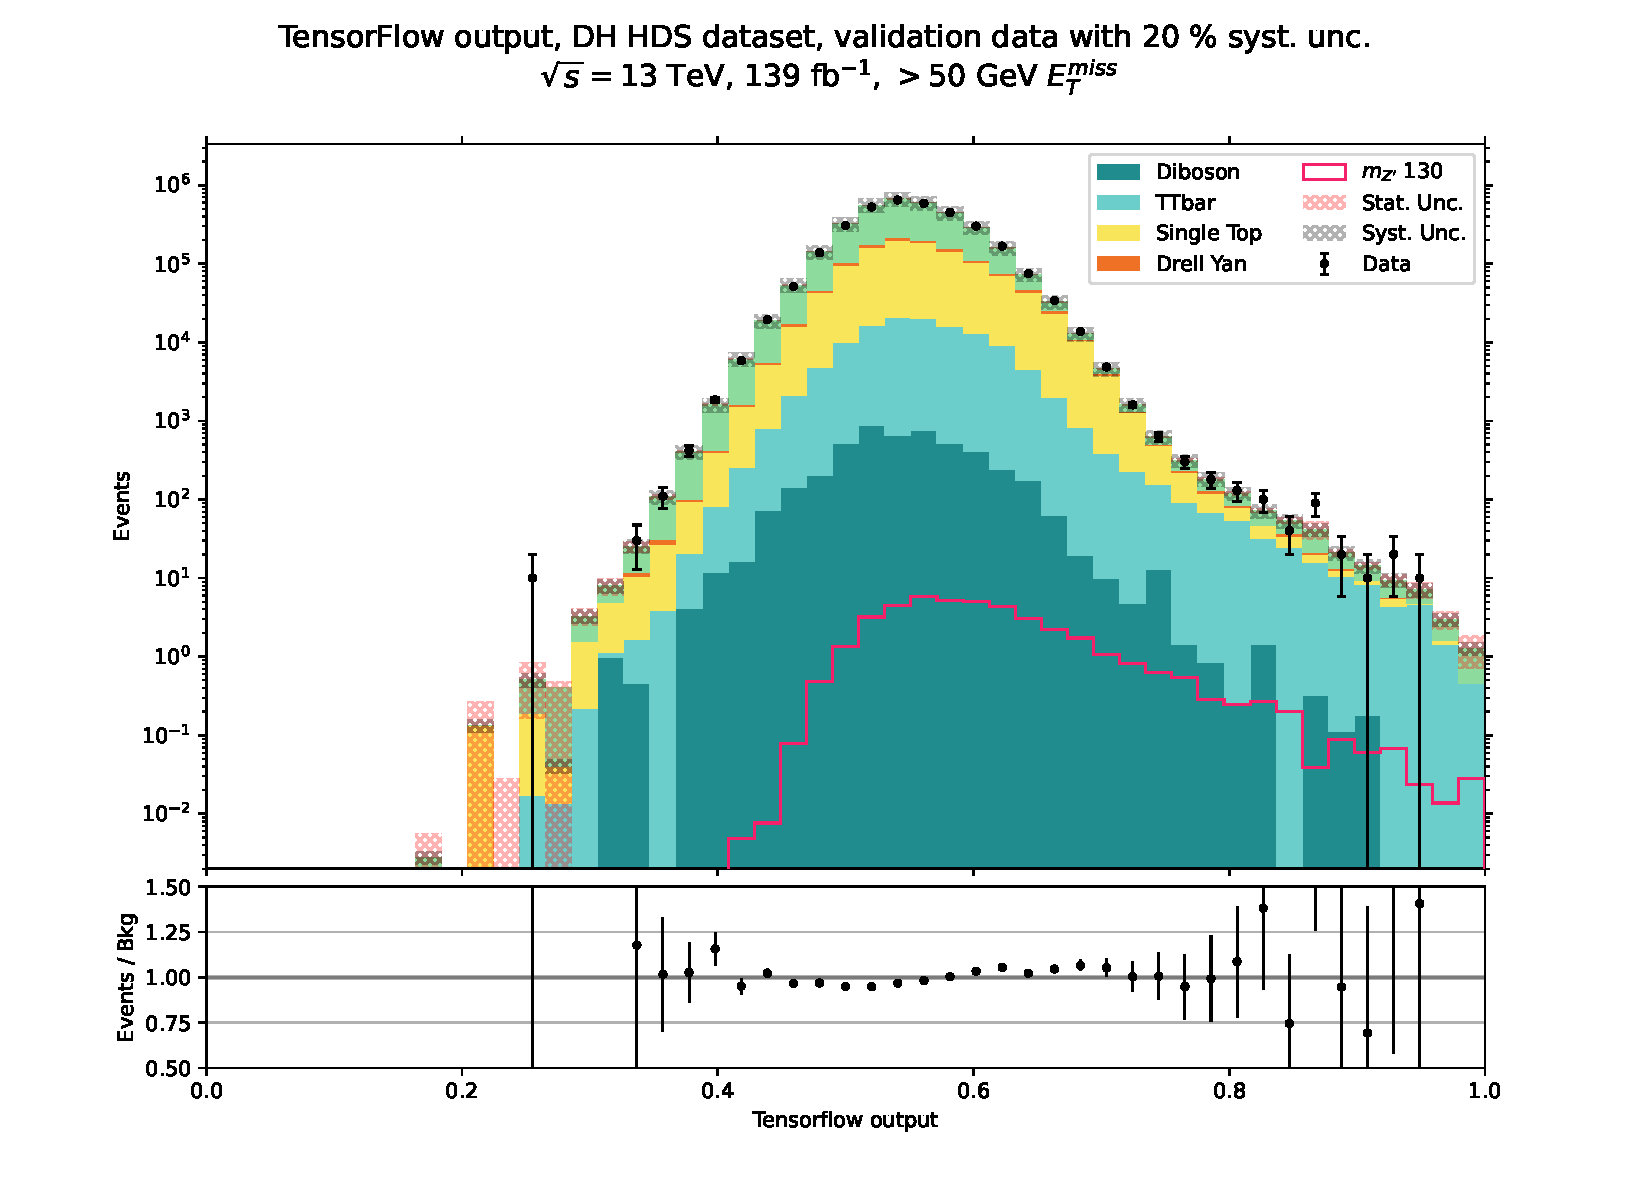
\includegraphics[width=1\textwidth]{New_pad/VAL.pdf}
      \caption{When including new features}
   \end{subfigure}
   \hfill
	\begin{subfigure}[b]{0.49\textwidth}
      \centering
      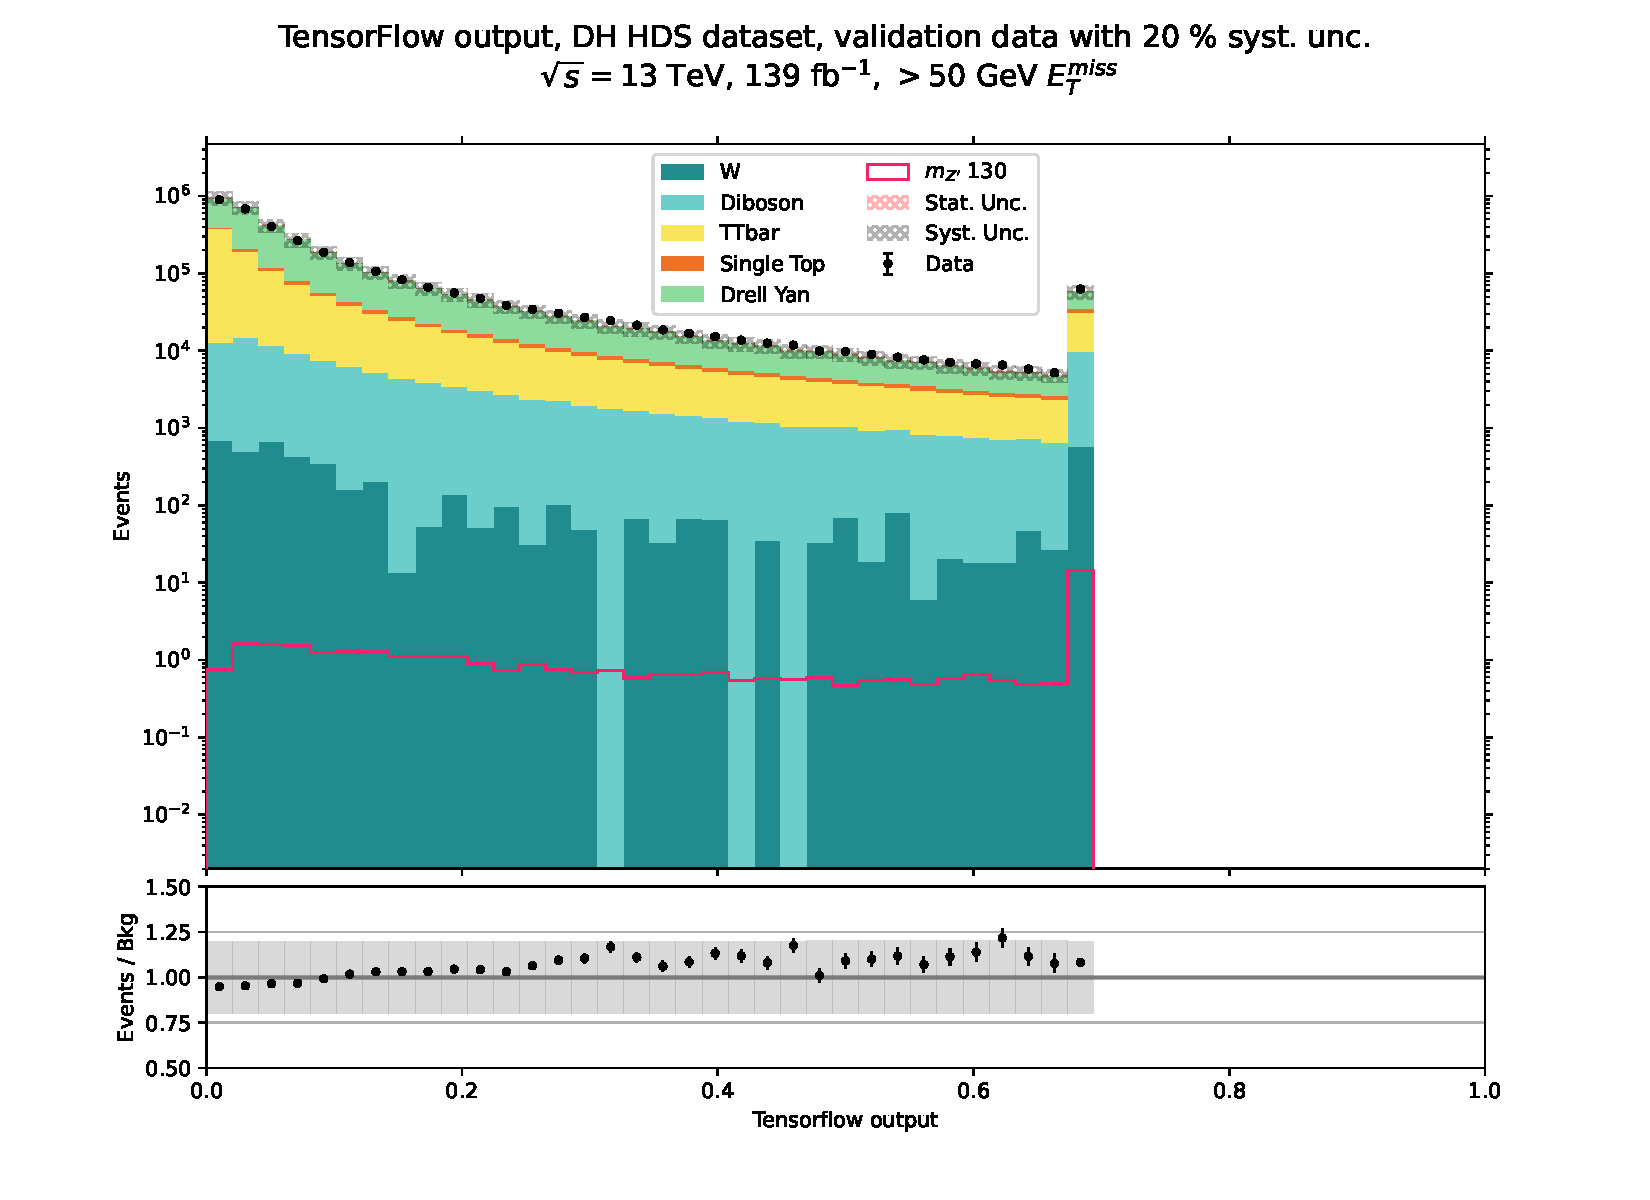
\includegraphics[width=1\textwidth]{No_pad/VAL.pdf}
      \caption{When dropping features}
   \end{subfigure}
   \caption[Validation plots for both padding methods]{Validation plots for both padding methods.  This is testing a dataset with 20\% of the Z' DH HDS $m_{Z'}=130$ GeV events.}\label{fig:NN_pad_VAL}
\end{figure}

% When I have however tested this and the difference in a optimized network (more info on this later) is minimal, and depending on our binning choice might make these new features less suited for our task. The resulta using 100 bins and using 50 bins 
% can be seen in Figure \ref{fig:New_var_pad}. For the remainder of our NN endevaours we will opt to not use these new features, and just remove the features that have missing variables all togheter.
% \graphicspath{{../../../Plots/NeuralNetwork/FULL/padding/}}
% \begin{figure}[!ht]
% 	\centering
% 	\begin{subfigure}[b]{0.49\textwidth}
%       \centering
%       \includegraphics[width=1\textwidth]{new_variables/finer_binning/VAL.pdf}
%       \caption{When including new variables and using 100 bins}
%    \end{subfigure}
%    \hfill
%    \begin{subfigure}[b]{0.49\textwidth}
%       \centering
%       \includegraphics[width=1\textwidth]{new_variables/finer_binning/EXP_SIG.pdf}
%       \caption{Expected significance of a)}
%    \end{subfigure}
%    \hfill
%    \begin{subfigure}[b]{0.49\textwidth}
%       \centering
%       \includegraphics[width=1\textwidth]{new_variables/VAL.pdf}
%       \caption{When including new variables and using 50 bins}
%    \end{subfigure}
%    \hfill
%    \begin{subfigure}[b]{0.49\textwidth}
%       \centering
%       \includegraphics[width=1\textwidth]{new_variables/EXP_SIG.pdf}
%       \caption{Expected significance of c)}
%    \end{subfigure}
%    \hfill
% 	\begin{subfigure}[b]{0.49\textwidth}
%       \centering
%       \includegraphics[width=1\textwidth]{no_pad/VAL.pdf}
%       \caption{When excluding new variables and using 50 bins}
%    \end{subfigure}
%    \hfill
%    \begin{subfigure}[b]{0.49\textwidth}
%       \centering
%       \includegraphics[width=1\textwidth]{no_pad/EXP_SIG.pdf}
%       \caption{Expected significance of e)}
%    \end{subfigure}
%    \caption[Network performace when testing new variables to avoid padding]{NN prediction when using new features to avoid padding. This is testing a dataset with a Z' DM model.}\label{fig:New_var_pad}
% \end{figure}

% \subsection{Grid Search}\label{sec:NNGriddy_res}
% The full results of the gridsearch when setting \verb|n_layers| = 2 (one hidden layer) and $\eta \in [0.001, 0.01, 0.1, 1]$, $\lambda\in[10^{-5},10^{-4},10^{-3},10^{-2}]$ and \verb|n_neuron|$\in[1, 10, 50, 100]$ can be found in my GitHub under \\\verb|Plots/NeuralNetwork/FULL/GRID_lamda_eta_neurons|, 
% but for the sake of this thesis not being too long I will only show the significance plot as well as the AUC for the testing and training set when setting $\lambda=10^{-5}$. 
% The significance is seen in Figure \ref{fig:NN_GRID_SIG}, while the AUC is in Figure \ref{fig:NN_GRID_AUC}.\\
% \graphicspath{{../../../Plots/NeuralNetwork/FULL/GRID_lamda_eta_neurons}}
% \begin{figure}[!ht]
%       \centering
%       \includegraphics[width=0.6\textwidth]{Significance_ne.pdf}
%       \caption{Grid search significance with $\lambda=10^{-5}$ and n\_layers = 2}\label{fig:NN_GRID_SIG}
% \end{figure}
% \graphicspath{{../../../Plots/NeuralNetwork/FULL/GRID_lamda_eta_neurons/AUC}}
% \begin{figure}[!ht]
% 	\centering
% 	\begin{subfigure}[b]{0.49\textwidth}
%         \centering
%         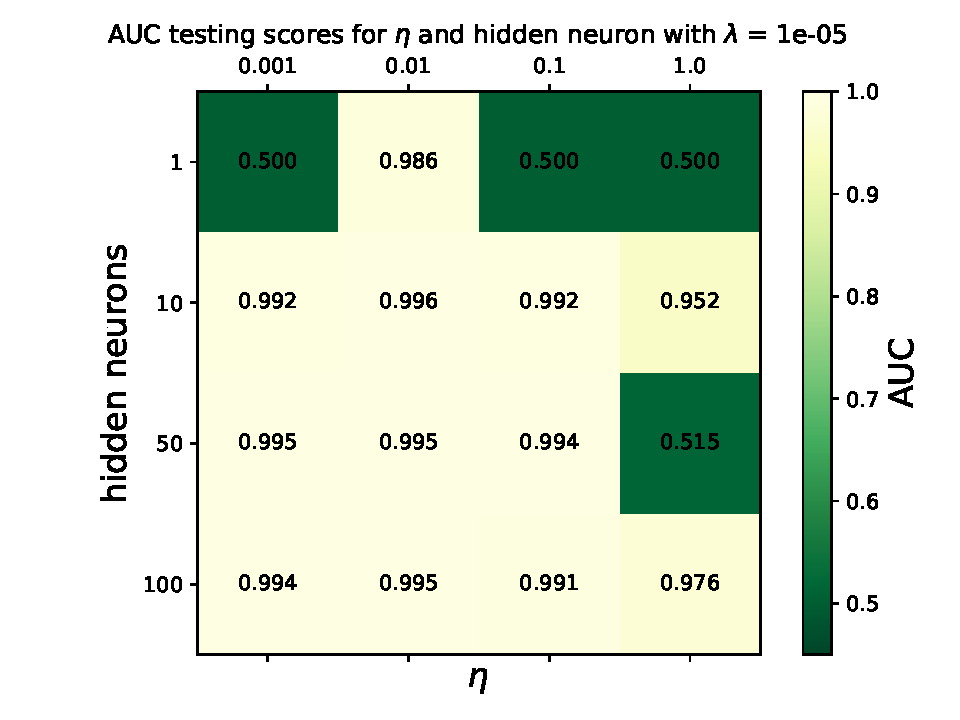
\includegraphics[width=1\textwidth]{testing_ne.pdf}
%         \caption{Testing AUC}
%      \end{subfigure}
%      \hfill
%      \begin{subfigure}[b]{0.49\textwidth}
%         \centering
%         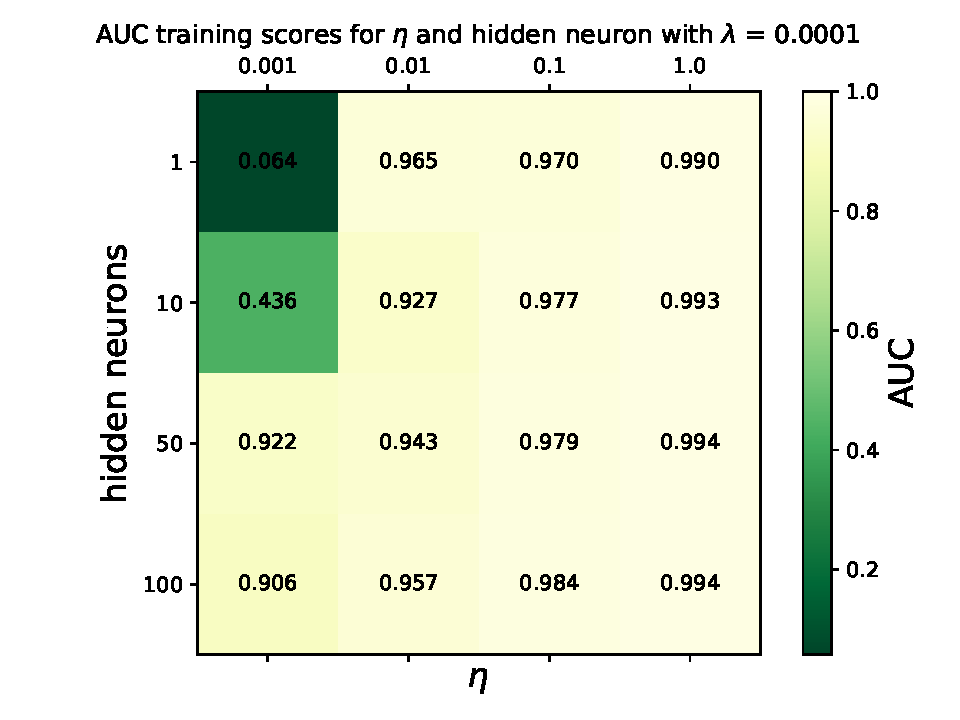
\includegraphics[width=1\textwidth]{training_ne.pdf}
%         \caption{Training AUC}
%      \end{subfigure}
%      \caption{Grid search AUC with $\lambda=10^{-5}$ and n\_layers = 2}\label{fig:NN_GRID_AUC}
% \end{figure}
% \newpage\noindent Doing the same but with more hidden layers and setting $\lambda=10^{-5}$ we get the results shown in GitHub under \verb|Plots/NeuralNetwork/FULL/GRID_layers_eta_neurons|, 
% for the sake of this thesis not being too long I will again only show the significance plot as well as the AUC for the testing and training set but this time when setting $\eta=0.01$. 
% The significance is seen in Figure \ref{fig:DNN_GRID_SIG}, while the AUC is in Figure \ref{fig:DNN_GRID_AUC}. 
% \graphicspath{{../../../Plots/NeuralNetwork/FULL/GRID_layers_eta_neurons}}
% \begin{figure}[!ht]
%       \centering
%       \includegraphics[width=0.6\textwidth]{Significance_nl.pdf}
%       \caption{Grid search significance with $\lambda=10^{-5}$ and and $\eta = 0.01$}\label{fig:DNN_GRID_SIG}
% \end{figure}

% \graphicspath{{../../../Plots/NeuralNetwork/FULL/GRID_layers_eta_neurons/AUC}}
% \begin{figure}[!ht]
% 	\centering
% 	\begin{subfigure}[b]{0.49\textwidth}
%         \centering
%         \includegraphics[width=1\textwidth]{testing_nl.pdf}
%         \caption{Testing AUC}
%      \end{subfigure}
%      \hfill
%      \begin{subfigure}[b]{0.49\textwidth}
%         \centering
%         \includegraphics[width=1\textwidth]{training_nl.pdf}
%         \caption{Training AUC}
%      \end{subfigure}
%      \caption{Grid search significance with $\lambda=10^{-5}$ and $\eta = 0.01$}\label{fig:DNN_GRID_AUC}
% \end{figure}
% \newpage\noindent I also made a test network with the same hyperparameters as the best one in Figure \ref{fig:DNN_GRID_SIG}, the only difference being that it has 10 hidden layers.
% I plotted the validation data to see how different the networks were at predicting the DH HDS $m_{Z'}=130$ GeV model. 
% These were trained and tested when using the Z-score normalization, Eq. (\ref{eq:Z-score}), and the weighting method explained in section \ref{sec:wgts}. The results are shown in the figure below.
% \graphicspath{{../../../Plots/DeepNeuralNetwork/FULL/BEST_GRID/DH_HDS_mZp_130/}}
% \begin{figure}[!ht]
% 	\centering
% 	\begin{subfigure}[b]{0.49\textwidth}
%         \centering
%         \includegraphics[width=1\textwidth]{VAL.pdf}
%         \caption{Four hidden layers}
%      \end{subfigure}
%      \hfill\graphicspath{{../../../Plots/DeepNeuralNetwork/FULL/10_HIDDEN_LAYERS/DH_HDS_mZp_130/}}
%      \begin{subfigure}[b]{0.49\textwidth}
%         \centering
%         \includegraphics[width=1\textwidth]{VAL.pdf}
%         \caption{Ten hidden layers}
%      \end{subfigure}
%    \hfill\graphicspath{{../../../Plots/DeepNeuralNetwork/FULL/BEST_GRID/DH_HDS_mZp_130/}}
%    \begin{subfigure}[b]{0.49\textwidth}
%       \centering
%       \includegraphics[width=1\textwidth]{EXP_SIG.pdf}
%       \caption{The expected significance of a)}
%    \end{subfigure}
%    \hfill\graphicspath{{../../../Plots/DeepNeuralNetwork/FULL/10_HIDDEN_LAYERS/DH_HDS_mZp_130/}}
%    \begin{subfigure}[b]{0.49\textwidth}
%       \centering
%       \includegraphics[width=1\textwidth]{EXP_SIG.pdf}
%       \caption{The expected significance of b)}
%    \end{subfigure}
%      \caption{Comparison of the network performance when having four and ten hidden layers. Figure a) and b) show the validation data of both cases, c) and d) show the expected significance of the validation plots when making a cut on the output. }
% \end{figure}
% \newpage\noindent This hints that we could be able to make a DNN with more hidden layers and get better results. However there are a few things that need to be noted when doing this, aside from the padding which is an even greater problem.
% The first and smallest one is that we could have used batch normalization instead of Z-score, but this is again something to be further discussed.\\
% \\The second being that I have not used the "balanced weighting" method when training the network, which might be for better or worse if the network really does ignore all EFT models...\\
% \\The third one which is more technical is that since more complex networks require more computational power, then this leads to us decreasing the batch size. Which lowers the statistics of signal, 
% and might even lead to the network training on batches without any signal sample at all. So the trade off is also something to be discussed.\\
% \\The last thing to be noted is that having a DNN completely removes the possibility of combining the results of multiple networks trained on a single model, as the imbalance becomes too much for the network to see anything.
% A solution to this however, is that instead of combining the results of multiple networks trained on a singular model, one could try the Parametrized NN approach used by Baldi et. al. \cite{Baldi_2016}, which could potentially avoid the imbalance problem, but this is 
% proposed as a plausible new research project due to time constrain on this thesis.
\clearpage




\section{Boosted Desicion Tree Training}
\subsection{Weights}
I have tried all of these options and the results can be seen in Figure \ref{fig:BDT_wgts}.\\
\\As we can see it makes a significant difference whether we use the weights to re-weight MC events to expected events. But there is no mathematical reason as to why we should 
include this re-weighting weight as sample weights, as the reason to use sample weights is to \textit{only} balance signal and bacgkround. In theory it makes no sense whatsoevert to include these weights either 
as the network doesn't really care for cross sections or luminosity, and what we are doing in principle is making it harder for the network to learn anything. But as seen on the results, the BDT learns the background 
extremely well when using the weights, while it also does a poorer job in learning the signal we are testing.\\ 
\\In a sense this is not a negative thing for our purposes, but stricly speaking we are invoking a semi-unsupervised learning method by punishing the network if it learns the signal too quickly. 
To get to the point as why this is good for our purposes, we are indirectly making our network more model indepentent! Because of this, the method that will be pursued further in this thesis will be to 
take the positive weights and balance the data.\todo{Add that ATLAS used it, so because of that so can I?}

\graphicspath{{../../../Plots/XGBoost/WEIGHT_TEST/DH_HDS_mZp_130/}}
\begin{figure}[!ht]
	\centering
	\begin{subfigure}[b]{0.49\textwidth}
      \centering
      \includegraphics[width=1\textwidth]{ATLAS_ABS/VAL.pdf}
      \caption{Using the scaled absolute value of the weights}
   \end{subfigure}
   \begin{subfigure}[b]{0.49\textwidth}
      \centering
      \includegraphics[width=1\textwidth]{POS/VAL.pdf}
      \caption{Using only positive weights}
   \end{subfigure}
   \begin{subfigure}[b]{0.49\textwidth}
      \centering
      \includegraphics[width=1\textwidth]{NONE/VAL.pdf}
      \caption{Using no weights}
   \end{subfigure}
   \caption[Difference when using different weighting methods on BDTs]{Difference when using different weighting methods. All networks were trained using the balancing method explained in Section \ref{sec:wgts}}\label{fig:BDT_wgts}
\end{figure}


\clearpage
\subsection{Grid Search}\label{sec:BDTGriddy_res}

\newpage\noindent As the previous results are to be taken with a heavy grain of salt, I conducted another grid search. On the second grid search I set the values of $\eta=0.1$ as the trend showed this giving the best results with less overtraining, 
and $\lambda=10^{-5}$ \todo{should I conduct a new grid search with different $\lambda$ and loss functions?}. This grid search had \verb|n_estimators| $\in[10, 100, 500, 1000]$ and depth $\in[3,4,5,6]$. 
The expected significance is shown in Figure \ref{fig:BDT_sig}. The testing and training AUC can be seen in Figure \ref{fig:BDT_GRID_AUC}.
\graphicspath{{../../../Plots/XGBoost/FULL/GRIDSEARCH_n_est_10-1000}}
\begin{figure}[!ht]
   \centering
   \includegraphics[width=0.6\textwidth]{Expected_significance.pdf}  
   \caption{Grid search expected significance when setting $\lambda=10^{-5}$ and $\eta=0.1$}\label{fig:BDT_sig}
\end{figure}
\begin{figure}[!ht]
\centering
\begin{subfigure}[b]{0.49\textwidth}
      \centering
      \includegraphics[width=1\textwidth]{Testing_AUC.pdf}
      \caption{Testing AUC}
   \end{subfigure}
   \hfill
   \begin{subfigure}[b]{0.49\textwidth}
      \centering
      \includegraphics[width=1\textwidth]{Training_AUC.pdf}
      \caption{Training AUC}
   \end{subfigure}
   \caption[Grid search result for BDT]{Grid search AUC when setting $\lambda=10^{-5}$ and $\eta=0.1$}\label{fig:BDT_GRID_AUC}
\end{figure}
\\When testing the best network with a depth of 6 and 1000 estimators on the same DH HDS $m_{Z'}=130$ GeV model we get the feature importance plots shown in Figure \ref{fig:BDT_feat}. 
Here we see that the "weight" metric gives us the expected features as most important. But the "cover" metric seems to be less of what we expect since the jet kinematic variables score higher, 
this might just be a curiosity rather than something to be suspect of.
\graphicspath{{../../../Plots/XGBoost/FULL/GRIDSEARCH_n_est_10-1000/DH_HDS_mZp_130/feature_importance/}}
\begin{figure}[!ht]
	\centering
   \begin{subfigure}[b]{0.8\textwidth}
      \centering
      \includegraphics[width=1\textwidth]{weight.pdf}
      \caption{Using "weight" metric}
   \end{subfigure}
   \hfill
   \begin{subfigure}[b]{0.8\textwidth}
      \centering
      \includegraphics[width=1\textwidth]{total_cover.pdf}
      \caption{Using "coverage" metric}
   \end{subfigure}
   \caption[Feature importance plots of BDT]{Feature importance of depth 6 network trained on FULL Z' DM data set when testing it on DH HDS $m_{Z'}=130$ GeV model.}\label{fig:BDT_feat}
\end{figure}


\end{document}